\documentclass[12pt, twoside]{article}
\linespread{1.15}
\usepackage[utf8]{inputenc}  % Ensure this is loaded before biblatex
\usepackage[sorting=none]{biblatex}  % Load the biblatex package
\addbibresource{./../Quellen/sources.bib}  % Add your .bib file


%%%%%%%%%%%%%%%%%%%%%%%%%%%%% Using Packages %%%%%%%%%%%%%%%%%%%%%%%%%%%%%%%%%%
\usepackage[a4paper, margin=2cm, top=5mm, includehead, headheight=2cm]{geometry}
\usepackage{graphicx}
\usepackage{amssymb}
\usepackage{amsmath}
\usepackage{amsthm}
\usepackage{empheq}
\usepackage{mdframed}
\usepackage{booktabs}
\usepackage{lipsum}
\usepackage{graphicx}
\usepackage{color}
\usepackage{psfrag}
\usepackage{pgfplots}
\usepackage{bm}
\usepackage{float}
\usepackage{wrapfig}
\usepackage{enumitem}
\usepackage[export]{adjustbox} % for valign option
\usepackage{caption}
\usepackage{subcaption}
\usepackage{hyperref}
\usepackage{array}
\usepackage{tocloft}
\usepackage[section]{placeins}
\usepackage[nottoc,numbib]{tocbibind}
\usepackage{ragged2e}
\usepackage{pdfpages}
\usepackage[autostyle=true,german=quotes]{csquotes}
\usepackage{siunitx}
\sisetup{locale = DE} 
\usepackage{emptypage}
\usepackage{fancyhdr}
\usepackage{booktabs}
\usepackage{tabularx}
\usepackage{array}
\usepackage{longtable}
\usepackage{multirow}


\usepackage{helvet}

\renewcommand{\familydefault}{\sfdefault}

\renewcommand{\footrulewidth}{0.4pt}%
\renewcommand{\headrulewidth}{0.4pt}%

\renewcommand{\headruleskip}{3mm}
\renewcommand{\footruleskip}{4mm}

\usepackage[main = ngerman, english]{babel}
\usepackage[ddmmyyyy]{datetime}

\newcommand{\todayD}{\the\day.\the\month.\the\year}   

\graphicspath{{../Bilder/}}

\setlength\parindent{0pt}
\counterwithin{figure}{section}
\counterwithin{table}{section}


\clubpenalty=10000
\widowpenalty=10000
\displaywidowpenalty=10000

\let\oldsection\paragraph
\renewcommand{\paragraph}[1]{\needspace{3\baselineskip}\oldsection{#1}}
%%%%%%%%%%%%%%%%%%%%%%%%%%%%%%%%%%%%%%%%%%%%%%%%%%%%%%%%%%%%%%%%%%%%%%%%%%%%%%%
\newcommand{\uni}[1]{\ensuremath{\, \mathrm{#1}}}
\DeclareSIUnit{\Umdrehung}{U}
% Other Settings
\usepackage[dvipsnames]{xcolor}

%\pagecolor[rgb]{0,0,0} %black

%\color[rgb]{0.5,0.5,0.5} %grey

%uncomment to make the links not display the red border
%\hypersetup{
%    colorlinks,
%    citecolor=black,
%    filecolor=black,
%    linkcolor=black,
%    urlcolor=black
%}

\sisetup{
detect-all
}


%% codestuff
\usepackage{listings, listings-rust}
\setlength{\parindent}{8pt}
\usepackage{indentfirst}
\definecolor{codegreen}{rgb}{0,0.6,0}
\definecolor{codegray}{rgb}{0.5,0.5,0.5}
\definecolor{codecomment}{rgb}{0.6,0.6,0.6}
\definecolor{backcolour}{rgb}{1,1,1}
\definecolor{lightgray}{rgb}{.9,.9,.9}
\definecolor{darkgray}{rgb}{.4,.4,.4}
\definecolor{codepurple}{rgb}{0.65, 0.12, 0.82}

\lstdefinelanguage{JavaScript}{
    backgroundcolor=\color{backcolour},   
    keywords={typeof, new, true, false, catch, function, return, null, catch, switch, var, if, in, while, do, else, case, break},
    keywordstyle=\color{NavyBlue},
    ndkeywords={class, export, boolean, throw, implements, import, this},
    ndkeywordstyle=\color{codegray},
    identifierstyle=\color{black},
    sensitive=false,
    comment=[l]{//},
    morecomment=[s]{/*}{*/},
    commentstyle=\color{codecomment},
    stringstyle=\color{codepurple}\ttfamily,
    morestring=[b]',
    morestring=[b]"
}

\lstdefinestyle{mystyle}{
    basicstyle=\fontsize{10}{12},
    backgroundcolor=\color{backcolour},   
    commentstyle=\color{codecomment},
    keywordstyle=\color{NavyBlue},
    numberstyle=\tiny\color{codegray},
    stringstyle=\color{codepurple},
    basicstyle=\ttfamily\footnotesize\bfseries,
    breakatwhitespace=false,         
    breaklines=true,                 
    captionpos=t,                    
    keepspaces=true,                 
    numbers=left,
    numbersep=5pt,                  
    showspaces=false,                
    showstringspaces=false,
    showtabs=false,                  
    tabsize=2
}
% -- Setting up the custom style:
\lstset{style=mystyle}

%%%%%%%%%%%%%%%%%%%%%%%%%% Page Setting %%%%%%%%%%%%%%%%%%%%%%%%%%%%%%%%%%%%%%%
\geometry{a4paper}

\newcommand{\iu}{{i\mkern1mu}}
\newcommand*\mathinhead[2]{\texorpdfstring{$\boldsymbol{#1}$}{#2}}

\definecolor{mred}{rgb}{0.619, 0.2392, 0.3176}


%%%%%%%%%%%%%%%%%%%%%%%%%%%%%%% Title & Author %%%%%%%%%%%%%%%%%%%%%%%%%%%%%%%%
\title{AFSS - Automated Factory Storage System}
\author{Benedikt Simbürger \\
    \and Nikolaj Voglauer \\
    \and Vincent Sonvilla \\
    \and Elena Widmann
    }

%%%%%%%%%%%%%%%%%%%%%%%%%%%%%%%%%%%%%%%%%%%%%%%%%%%%%%%%%%%%%%%%%%%%%%%%%%%%%%%
\babelprovide[import]{ngerman}


\fancyhf{}

\fancyhf[EHL]{\includegraphics[width=0.2\textwidth]{HTL_Moessingerstraßen_Logo.png}}
\fancyhf[OHL]{\includegraphics[width=0.2\textwidth]{HTL_Moessingerstraßen_Logo.png}}

\fancyhf[EHC]{\begin{tabular}{cc}
    Simbürger & Sonvilla \\
    Voglauer & Widmann \\
\end{tabular}}

\fancyhf[OHC]{\begin{tabular}{cc}
    Simbürger & Sonvilla \\
    Voglauer & Widmann\\
\end{tabular}}


\fancyhf[EFL]{\todayD}
\fancyhf[EFR]{\thepage}
\fancyhf[EHR]{\color{mred} ELEKTROTECHNIK}


\fancyhf[OFR]{\todayD}
\fancyhf[OFL]{\thepage}
\fancyhf[OHR]{\color{mred} ELEKTROTECHNIK}

\fancyhf[EFC]{Automated-Factory-Storage-System}
\fancyhf[OFC]{Automated-Factory-Storage-System}

\raggedbottom

\begin{document}

\pagenumbering{gobble}

\setlength{\parindent}{0pt}

\begin{figure}[h]
    \vspace{-5mm}
    \includegraphics[width=0.5\textwidth]{HTL_Moessingerstraßen_Logo.png}
    \centering
\end{figure}

\begin{center}
    \Large \textbf{HÖHERE TECHNISCHE BUNDESLEHRANSTALT} \\
    \vspace{5mm}
    \Large{KLAGENFURT, MÖSSINGERSTRASSE}

\end{center}

\vspace{7mm}

\begin{center}
    \Large{ABTEILUNG ELEKTROTECHNIK}
\end{center}

\hrule

\vspace{10mm}

\begin{center}
    \Huge \textbf{DIPLOMARBEIT} \\
    \vspace{7mm}
    \huge{Titel der Diplomarbeit Deutsch}

    \vspace{7mm}
    \huge{Automated-Factory-Storage-System}

    \vspace{7mm}
    \Large{JAHRGANG 5AHET}

\end{center}

\vspace{15mm}

\begin{flushleft}
    \linespread{1}
    \bgroup
        \large
        \def\arraystretch{1.5}
        \begin{tabular}{p{5cm}l}
            eingereicht von & Benedikt Simbürger\\
            & Vincent Sonvilla\\
            & Nikolaj Voglauer\\
            & Elena Widmann\\
            Projektbetreuer & Dipl.-Ing. Christian Sallinger
        \end{tabular}
    \egroup
\end{flushleft}

\vspace{7mm}
\large
Diese Diplomarbeit entspricht den Standards gemäß dem Leitfaden zur Umsetzung der Reife- und Diplomprüfung des BMBWF in der letztgültigen Fassung.\par
\begin{flushright}
    Klagenfurt, am 04.04.2025
\end{flushright}

\newpage

\begin{figure}[h]
    \includegraphics[width=0.5\textwidth]{HTL_Moessingerstraßen_Logo.png}
    \centering
\end{figure}

\begin{center}
    \huge \textbf{EIDESSTATTLICHE ERKLÄRUNG}\\
    \vspace{7mm}
    \large
    \begin{tabular}{p{14cm}}
        Ich versichere an Eides statt, dass ich diese Diplomarbeit
        selbstständig verfasst und keine anderen als die angegebenen
        Quellen und Hilfsmittel verwendet habe. Alle Gedanken, die im
        Wortlaut oder in grundlegenden Inhalten aus unveröffentlichten
        Texten oder aus veröffentlichter Literatur übernommen, oder mit
        künstlicher Intelligenz generiert wurden, sind ordnungsgemäß
        gekennzeichnet, zitiert und mit genauer Quellenangabe
        versehen.
    \end{tabular}

    \vspace{10mm}
    Verfasser/Verfasserin\\
    
    \vspace{40mm}
    \bgroup
        \newcolumntype{P}[1]{>{\centering\arraybackslash}p{#1}}
        \def\arraystretch{1.5}
        \begin{tabular}{P{67mm}p{14mm}P{67mm}}
            \cline{1-1}
            \cline{3-3}
            Benedikt Simbürger & & Vincent Sonvilla\\
        \end{tabular}

        \vspace{35mm}
        \begin{tabular}{P{67mm}p{14mm}P{67mm}}
            \cline{1-1}
            \cline{3-3}
            Nikolaj Voglauer & & Elena Widmann\\
        \end{tabular}
    \egroup

    \vspace*{\fill}
    \raggedleft Klagenfurt, am 04.04.2025

\end{center}

\newpage

\pagestyle{fancy}
\pagenumbering{arabic}
\normalsize

\section*{Kurzbeschreibung}

Das Bauteillager der Werkstätte der HTL-Mössingerstraße, ist aktuell eine Kombination aus Schränken und Facher, bei welchen von Hand Ein- und Ausgelagert werden muss. Da dies sehr Zeitaufwändig und Fehleranfällig ist, soll eine automatische Lösung abhilfe schaffen. \\ \\
Ziel des Projekts "Automated-Factory-Storage-System" ist es, eine Gesamtlösung für ein automatische Kleinteillagersystem, nach dem Vorbild der Industrie zu entwickeln. So soll unter anderem ein Realitätsbezug vom im Unterricht gelernten zu schaffen. Deshalb werden auch alle Steuerungskomponenten, so industrienahe wie möglich ausgeführt.



\subsection*{Aufgabenstellung}
\begin{itemize}
    \item Warum ist die Themenstellung von Interesse?
    \item Was ist die vorgegebene Zielsetzung?
    \item Welche Ergebnisse sind zu erreichen?
\end{itemize}

\subsection*{Realisierung}
\begin{itemize}
    \item Von welchem Stand der Technik im Umfeld der Aufgabenstellung wurde ausgegan-gen?
    \item Welche Lösungsansätze sind grundsätzlich möglich?
    \item Warum wurde ein bestimmter Lösungsansatz gewählt?
    \item Welche experimentelle, konstruktive oder softwaretechnische Methodik wurde angewendet?
    \item Auf welche fachtheoretischen Grundlagen wurde aufgebaut?
    \item Welche wirtschaftlichen Überlegungen wurden angestellt?
\end{itemize}

\subsection*{Ergebnisse}
\begin{itemize}
    \item Worin besteht der konkrete Beitrag zur Lösung der Aufgabenstellung (Prototyp, Entwurfsplanung, Softwareprodukt, Businessplan etc.)?
    \item Kann das Ergebnis durch eine typische Grafik, ein Diagramm bzw. ein Foto illus-triert werden?
    \item Kann in die Vollversion der Diplomarbeit Einsicht genommen werden?
\end{itemize}

\color{black}
\vspace*{\fill}
\section*{}

\bgroup
    \def\arraystretch{1.5}
    \begin{tabular}{p{48mm}p{113mm}}
        \textbf{Kurztitel:} & \textcolor{blue}{Kurztitel der Diplomarbeit (etwa. 30 Zeichen)}\\
        \textbf{Schlüsselwörter:} & \textcolor{blue}{Maximal fünf aussagekräftige und durch Kommas getrennte Schlüsselwörter, welche die Inhalte möglichst gut beschreiben.}
    \end{tabular}
\egroup

\newpage

\section*{Abstract}
\textcolor{blue}{Die Kurzbeschreibung in englischer Sprache sollte sinngemäß exakt der Kurzbeschreibung in deutscher Sprache entsprechen, siehe Abschnitt „Kurzbeschreibung“.}

\vspace*{\fill}
\section*{}

\bgroup{}
    \def\arraystretch{1.5}
    \begin{tabular}{p{48mm}p{113mm}}
        \textbf{Short title:} & \\
        \textbf{Keywords:} & 
    \end{tabular}
\egroup{}

\newpage

\tableofcontents
\newpage
\section{Allgemeiner Teil}

\subsection{Ausgangssituation 1-2}

\subsubsection{Anforderungen 1/2}



\subsection{Potentielle Lösungen 2}
\subsubsection{Lagermethoden 3/4}

\subsubsection{Steuerung 4/9}

\subsubsection{Schaltschrank 4/9}


\subsection{Verfolgter Lösungsansatz 3/4}


\subsection{Methodik 5}

\subsubsection{Software 2}

\subsubsection{Hardware 2}

\subsubsection{Fertigung 1}

\subsection{Sicherheitstechnik 1}

\subsection{Kooperationspartner}

\newpage

\color{black}
\newpage
\fancyhf[OHC]{
    \centering
    Benedikt Simbürger
}
\fancyhf[EHC]{
    \centering
    Benedikt Simbürger
}


\section{Hardwareentwicklung, Softwarebackend \\ und Benutzeroberfläche \textcolor{gray}{(Simbürger)}}

\subsection{Hardware}

\subsubsection{Planung}
Grundlegende Anforderungen zur planung der AFSS-Mechanik, sind die größe des Lifts an der \\HTL-Mössingerstraße, sowie möglichst einfache realisierung mit HTL-mitteln, möglichst wenig kompromisse in der Funktion oder zuverlässigkeit eingehen zu müssen.
Die Anforderung der Transportfähigkeit limitiert die Größe des Lagers auf 2.3 m Länge um im Lift transportiert werden zu können und auf 1.9 m höhe aufgrund der Türhöhe im Keller. Weiters müssen auch noch Rollen an den Rahmen angebracht werden, um das Lager überhaubt erst ohne großen mehraufwand bewegen zu können. Diese Extrahöhe limitiert den Rahmen weiter.
Nun soll dieser rund 2.25 m lange und 1.8 m hohen Raum optimal genutzt werden um eine möglichst große Lagerdichte sicherstellen zu können.
Um möglichst gute erweiterbarkeit, sowie eine Fertigung an der Schule zu ermöglichen, sollen für die mechanische Trägerkonstruktion sog. Item-Profile verwendert werden. 

\paragraph{Item}

\begin{wrapfigure}{r}{0.3\textwidth}
    \vspace{-5mm}
    \includegraphics[width=0.3\textwidth]{Item-Standartverbindungssatz.png}
    \caption{Item Profil mit Standartverbindungssatz \cite{Item_svs}}
\end{wrapfigure}

Das Item-Profilsystem, ist ein System welches Aluminium Extrusionen in verschiedenen Ausführungen, sowie viele Verbindungs-möglichkeiten zu sich selbst sowie andere mechanische Elemente bietet. Hierbei gibt es eine breite Auswahl an Profielen, von 20x20 mm bis 40x40 mm Querschnitt. Für alle Komponenten mit hoher mechanischer Beanspruchung werden 40x40-Extrusionen verbaut, da diese eine besonders hohe Biegefestigkeit aufweisen. Für Anwendungen mit geringerer Beanspruchung sowie aus Platz- und Gewichtsparmaßnahmen, werden 20x20-Extrusionen Verbaut. 
Zur Verbindung zu anderen Bauelementen gibt es die Möglichkeit sog. Nutenstene mit verschiedenen Gewinden in die Nut einzulegen und dort Platten o. ä. anzuschrauben. Um Item-Profile untereinander zu verbinden, werden Standartverbindungssätze verwendet. 
\\
Die Anwendung im AFSS erfordert weiters recht lange Verfahrwege. Um dies kostengünstig umsetzen zu können, werden V-Slot Profile verwendet


\paragraph{V-Slot}

\begin{wrapfigure}{r}{0.3\textwidth}
    \vspace{-5mm}
    \includegraphics[width=0.3\textwidth]{V-Wheel.png}
    \caption{V-Slot mit V-Wheel \cite{v_slot_wheel}}
\end{wrapfigure}

Auch V-Slot-Profile sind Aluminium Extrusionen. Diese können grundsätzlich auch ähnlich wie Item-Profile, mit Nutensteinen ect. verwendet werden, sind aber zusätzlich darauf ausgelegt, dass ein V-Wheel in einer Narbe des Profils rollen kann. 




\subsubsection{Rahmen}

Der Rahmen des AFSS bezeichnet jene Struktur, welche als äußerstes Gehäuse, sowie grundlegende mechanische Stabilität bietet. Es ist geplant, dass es die anforderungen von Maximalhöhe und -länge optimal ausnutzt sowie breite minimal hält.  

\subsubsection{Y-Achse}
\paragraph{Motorauslegung}

\subsubsection{X-Achse}
Die X-Achse des AFSS is 


\paragraph{Schlittenauslegung}



\paragraph{Antrieb}

\paragraph{Kabelführung}


\subsubsection{Z-Achse ("Gabel")}
\paragraph{Positionsbestimmung}

Um die optimale Postiton der Zahnriemenaufhängung für die Y-Achse bestimmen zu können, wird überschlagsmäßig ein Massenschwerpunkt in Z-Richtung berechnet. Um die Konstrukiton beginnen zu können, werden hierfür ungefähre werte angenommen.

\noindent\begin{minipage}{\textwidth}
\begin{minipage}[t]{0.5\textwidth}
    \vspace{7mm}
    \begin{equation*}
        X_s = \frac{1}{M} \cdot \displaystyle\sum_{i = 0}^{n} z_i \cdot m_i
    \end{equation*}
\end{minipage}%
\begin{minipage}[t]{0.5\textwidth}
    \begin{align*}
        &Z_s: \text{Z-Koordinate des Massenschwerpunkts} & &\left[m\right]\\
        &M: \text{Gesamtmasse} & &\left[kg\right]\\
        &z_1: \text{Z-Koordinate der Teilmasse} & &\left[m\right] \\
        &m_1: \text{Masse der Teilmasse} & &\left[kg\right]
    \end{align*}
\end{minipage}
\end{minipage} 
\vspace{5mm}

    \begin{table}[h!]
        \centering
        \centering
            \begin{tabular}{c c c}
                Gegenstand & Masse in kg & Position in mm\\
                \hline
                Motor & 0.3 & 21 \\
                Z-Schiene & 1 & 150 \\
                Z-Gable & 0.3 & 180 
            \end{tabular}
        \caption{X-Achse unbeladen und eingefahren}
        \end{table}
    \begin{table}[h!]
            \centering
            \begin{tabular}{c c c}
                Gegenstand & Masse in kg & Position in mm\\ 
                \hline
                Motor & 0.3 & 21 \\
                Z-Schiene & 1 & 150 \\
                Z-Gabel & 1.3 & 380
            \end{tabular}
            \caption{X-Achse beim Ladevorgang}
        \end{table}

        \vspace{5mm}
        So werden zwei Schwerpunkte berechnet: ca. 130 mm im unbeladen und 250 mm während dem Ladevorgang. Da die Stabilität des Y-Schuttels während dem Ladevorgang wichtiger ist als während einer Leerfahrt wird das Y-Shuttle so positioniert, dass die Aufhängung des Zahnriemen bei rund 200 mm liegt. 
    

\subsubsection{Fertigung}

\paragraph{Umlenkrollen}
Die Umlenkrollen sind jeweils am Ende der X- und Y-Achsen angebracht. Dadurch dass diese der gesamten Spannkraft ausgesetzt. Dies erfordert spezielle Anforderungen an die Aufhängen als auch an die Umlenkrolle selbst. Diese soll primär eine 180° Wende des Zahnriemens ermöglichen, sowie sekundär eine Führung für den Riemen bieten. 
Umgesetzt wird diese Anforderungen, durch Fertigung von vier Aluminium-Drehteilen in welche Kugellager eingepresst werden.

\begin{figure}[h]
    \centering
    \begin{subfigure}{.6\textwidth}
        \centering
        \includegraphics[width=10cm]{AT5x16-Umlenkung.png}
        \caption{Bauteilzeichnung Umlenkrolle}
        \label{UmlenkrolleBTZ}
        
    \end{subfigure}%
    \begin{subfigure}{.4\textwidth}
        \centering
        \includegraphics[width=5cm]{AT5x16-Umlenkung-Dorn.png}
        \caption{Dorn}
        \label{DornBTZ}
    \end{subfigure}
    %\caption{Dorn}
    %\label{fig:test}
    \end{figure}

Die Fertigung dieses Teils Lässt sich in folgende Teilschritte unterteilen:
\begin{itemize}
    \setlength\itemsep{0mm}
    \item Zuerst die Frontfläche Plandrehen (900 U/min)
    \item Ungefär 30mm Länge auf das Aussenmaß von 36mm Plandrehen
    \item Mit 9.8mm Bohrer das mittlere Loch vorbohren (540 U/min)
    \item Mit 10mm Reibeisen und viel Öl das Loch auf eine genaue passung bringen (260 U/min)
    \item Die Position Relativ zum Backenfutter makieren um beim neu einspannen Rundlaufgenauigkeit gewährzuleisten
    \item Zylinder bei ca. 26 mm Abstechen (540 U/min)
    \item Umspannen und auf maß plandrehen (900 U/min)
    \item Die Aussparung für die Lager mit Eckdrehmeissel beginnen, jedoch nach innen hin nur 6.8 mm 
    \item Bei ca. 17 mm Lochdurchmesser den tatsächleichen Durchmesser mit der Digitalanzeige vergleichen und gegebenennfalls korrigieren
    \item Bei 21.5 mm den Oberschlitten die restlichen 0.2 mm zustellen und die gesamte Tiefe plandrehen
    \item Den Lochdurchmesser auf 21.95 erweitern, und dann in kleinen inkrementen zustellen bis das Lager gerade so nicht passt, um einen Pressitz zu gewährleisten, dies tritt bei Lagern mit 22 mm Aussendurchmesser bei rund 22.04 mm ein.
    \item Da für die Einsparung der Riemenführungsfläche kein Angriffspunkt verfühbar ist wurde auls Halterung ein Dorn gedreht, auf welchen das Drehteil aufgeschraubt wird.
    \item Mit dem Abstechmeisel wird in 2 mm inkrementen die Zahnriemenauflagefläche herausdrehen, bis auf 30.2 mm, sowie links und rechts den Rand 1mm extra dick lassen. (540 U/min)
    \item Am Schluss wird der Rand auf Maß gedreht und die Tiefe fertiggedreht. 
    \item Als letzten Schritt werden links und rechts die zwei lager eingepresst.
\end{itemize}

    Durch die Verhältnissmäßig großen Toleranzen bei den Lageraussendurchmessern wird bei 2 der 8 Lagerpassungen zusätztlich Lagerkleber verwendet um eine Zuverlässige Passung zu gewährleisten.


\paragraph{Lasern}
\paragraph{Fräsen}

\subsubsection{Aufbau}

\subsection{Software und Benutzeroberfläche}

\subsubsection{Grundlegendes}

\subsubsection{Aufbau}

\subsubsection{Benutzeroberfläche}



\subsubsection{Datenbanken}

Als Datenbanksystem wird aufgrund des guten Supports MySQL gewählt. Dies ist ein relationales Datenbankmanagementsystem welches in einem Docker-Container aufgesetzt wird. In diesem werden alle Daten gespeichert, die zur Auswahl sowie zur Ausliferung von Teilen nötig sind.

\begin{figure}[h]
    \includegraphics[width=0.6\textwidth]{DB-Schema.png}
    \centering
    \caption{Datenbankschema des AFSS}
\end{figure}

Wie in Abb. 4.2 ersichtlich, beinhäklt sich diese Datenbank fünf Tabellen. Diese hohe Komplexität resultiert daraus, dass diese Struktur eine 100\%ige Flexivilität in der Ablage von Bauteilen in einem überliegendem System bietet.

Die Erste Tabelle beschreibt ein einziges theoretisches Bauteil. Dieses hat einen Namen, Gewicht, Beschreibung und Kategorien zur Filterung. Unter der Spalte 'picture' wird ein Dateiname gespeichert, der zu einem Bild zeigt, dass das Produkt abbildet.
Die zweite beschreibt einen Container. Im Lagersystem entspricht dieser einer Box. Diese kann mehrere `stocks' beinhalten, sowie durch einen Barcode identifiziert werden. Weiters muss jeder Container immer eine aktuelle Position (`current\_location') besitzen, an der die Box gerade ist. Im ausgelagerten (und noch nicht eingelagerten) Zustand ist diese `location' Position 0. Das Ziel der Box wird in `target\_location' gespeichert. Stimmt die aktuelle mit der Zielposition überein, so ist die Box an ihrem Ziel angelangt. Die Kategorie `size' beschreibt die Größe eines Containers und lässt somit theoretisch zu, dass in Zukunft auch unterschiedlich große Boxen zuverlässig in die richtigen Lagerplätze eingelagert werden. `priority' wird nicht verwendet.

Container und Artikel werden im sog. 'stock' verheiratet. Dieser kann als bauteilhaufen in einer Box verstanden werden. Es können also auch mehrere 'stocks' mit dem selben Container geben, dies würde mehreren verschiedenen Bauteilen in einem einzigen Copntainer entsprechen. Auch ist es möglich mehrere Container mit den selben 'stocks' abzubilden, welches ener aufteilung von Abuteilen auf mehrere Container entspräche.

Die Positionen der Container werden in Standorte ('locations') abgebildet. Diese entsprechen den Lagerplätzen. Sie sind einer darüberliegenden 'area' zugeordnet, welche einerseits einen Lagerschrank, aber weiters auch Module wie Vereinzelungsanalgen, abbilden kann. Standorte verfüghen weiters über eine Position welche in X, Y und Z-Richtung beschreibt, wo sich ein Standort im Referenzsystem des Lagers befindet. Auch die größe des Lagerplatzes wird abgebildet, um sicherzustellen, dass auf jeden fall nur die richtige Größe an Box eingelagert wird.


\subsubsection{Docker}

    \begin{wrapfigure}{r}{0.3\textwidth} % 'r' for right, 'l' for left
        \vspace{-20px}
        \includegraphics[width=0.3\textwidth]{docker-logo-011.png} % Replace with your image file
        \caption{Docker-Logo: \cite{docker_logo}}
    \end{wrapfigure}

    Docker ist eine Umgebung, in der Softwareprojekte isoliert werden können. Da besonders auch bei Projekten mit großem Python anteil, viele Pakete mit verschiedenen Versoinen benötigt werden, ist es sehr hilfreich diese zu bündeln. \\
    Umgesetzt wird dies mithilfe von Containern welche einen gesamten Programmteil als alleinstehende Einheit enthält. Diese werden über ein 'Dockerfile' configuriert, welches sich im selben Ordner wie die Python-Anwendung befindet. In diesem werden Parameter wie die Python-Version und die benötigten pip-Pakete sowie den Programmeinstiegspunkt angegeben. \\ 
    Ein zweier Docker Conteianer wird mit einem MySql-Image erstellt, dort wird die Datenbank aufgesetzt. \\
    Um diese Zwei Container miteinander Kommunizieren zu lasen, ist es ntig ein sog. docker-compose.yml File zu erstellen. Dies enthält alle Informationen über verwendete container, deren Ports, sowie Speicher für Dateien (Volumes). Bei Testbetrieb wird der Datenbankcontainer aleinstehend bestrieben und mit einem anderen Port, keine Zugriffsprobleme zu generieren. In Produktion wird dann derselbe Container in den Containerverband übertragen und dort mit einem anderen Port weiterverwendet. \\
    Erstellt wird dieser Containerverband mit den Consolenbefehlt der auf das docker-compose File zugreift. 
    \begin{lstlisting}[language=bash]
        docker build docker-compose.yml\end{lstlisting}
    Dann werden auch alle Logs in der Kommandozeile ausgegeben sowie 


\subsubsection{Backend}
\subsubsection{APIs}
\subsubsection{Lageralgorithmus}
\subsubsection{Artikelsuche}
\paragraph{TF-IDF und Rust Implementierung} \hspace{0pt} \\
Der TF-IDF (Term Frequency-Inverse Document Frequency) Algorithmus, ist ein Weg um wichtige wörter aus Dokumenten zu extrahieren. Er wird verwendet um beispielsweise in Suchmaschienen, eine Suchanfrage mit Webpagecontent abzugleichen, und die am besten mit der Suchanfrage übereinsteimmenden Dokumente zu sortieren. \\
Im Fall dieser Anwendung werden die Daten aus der Artikeldatenbank als 'Dokumente'  angesehen und die Suchanfrage aus dem Suchfeld wird dafür verwendet um die am besten passenden Artikel zu finden.
\\
Durch den Relativ hohen Rechenaufwand bei dieser Suchoperation wird dieser in der Programmiersprache Rust implementert. Die Implementierung in Rust ist im vergleich zu Python schon bei relativ kleinen Datenmenge bis zu 5-mal schneller.

\subparagraph{Rust}
Rust ist eine sehr effiziente und schnelle Programmiersprache die in den späten 2000er und frühen 2010ern bei Mozilla und der Open-Source-Community entwickelt. Sie unterstützt unter anderem mehr Typensicherheit und verhindert viele Programmierfehler. 

Die Funktion dieses Algorithmus ist in drei unterteile Unterteilt.

\begin{enumerate}
    \item Term Frequenz \\
    Die Termfrequenz gibt an, wie oft ein angegebenes Wort in einem Dokument vorhanen ist. Dies wird durch die Folgende Funktion kalkuliert.
    
    \begin{lstlisting}[language=Rust]
fn term_frequency(document: &str, term: &str) -> f64 {
    // Store the lowercase document as a String to ensure it lives long enough
    let lower_document = document.to_lowercase(); 

    // Split the document into words
    let normalize_document: Vec<&str> = lower_document.split_whitespace().collect();
    // Make sure the searchterm is lowercase
    let normalize_term = term.to_lowercase();

    // Count occurrences of the term in the document
    let count = normalize_document
        .iter()
        .filter(|&&word| word == normalize_term) // Compare each word with the term
        .count();

    // Calculate the term frequency as occurrences / total number of words
    let total_words = normalize_document.len();
    if total_words == 0 {
        0.0 // Avoid division by zero if the document is empty
    } else {
        count as f64 / total_words as f64
    }
}\end{lstlisting}

    Mithilfe dieser wird eine Liste aller Wörter und der Vorkommenshäufigkeit dieser erstellt.

    \item Die zweite Komponente ist dann die Inverse Dokument Frequenz. Diese gewichtet, die Anzahl der Dokumente in dem das gesuchte Wort enthalten ist relativ zur Gesamtdokumentanzahl vorkommt. Häufig vorkommende Worte wie z.B. 'und' werden hierbei weniger gewichtet als einzigartige Wörter.

\begin{lstlisting}[language=Rust]
fn inverse_document_frequency(term: &str, all_documents: &Vec<String>) -> f64 {
    let mut num_documents_with_this_term = 0;

    // Iterate over all documents to check if they contain the term
    for doc in all_documents {
        // Normalize both term and document by converting them to lowercase
        let lower_doc = doc.to_lowercase();
        let normalized_doc: Vec<&str> = lower_doc.split_whitespace().collect();

        // Check if the term exists in the document
        if normalized_doc.contains(&term.to_lowercase().as_str()) {
            num_documents_with_this_term += 1;
        }
    }

    // Calculate IDF
    if num_documents_with_this_term > 0 {
        // Apply the IDF formula: 1 + log(total_documents / documents_with_term)
        1.0 + ((all_documents.len() as f64) / (num_documents_with_this_term as f64)).ln()
    } else {
        // If the term is not found in any document, return 1.0
        1.0
    }
}
\end{lstlisting}

    \item Nun liegt Liste davon vor, wie oft ein Wort in den Suchdaten vorkommt, als auch, wie oft ein Suchbegriff in einem bestimmten Dokument ist. \\ Als nächsten Schritt werden diese beiden Werte für jeden Suchbegriff miteinander multipliziert und ergeben somit einen Vektor der die Suchwörter in Relation zu jedem einzelnen Dokument stellt.
    \item Als letzten Schritt wird der zuvor errechnete Dokumentenvektor (der IDF jedes Suchterms in jedem Dokument) mit dem Suchvektor verglichen. Die geschieht mit der sog. Kosinus-Ähnlichkeit.
    \begin{lstlisting}[language=Rust]
fn cos_similarity(query_p: Vec<f64>, document_p: Vec<f64>) -> f64 {
    // Ensure that both vectors have the same length
    if query_p.len() != document_p.len() {
        return -1.0;
    }

    let mut dot_product = 0.0;
    let mut abs_doc_squared = 0.0;
    let mut abs_query_squared = 0.0;

    // Calculate the dot product and the magnitudes (squared)
    for i in 0..query_p.len() {
        dot_product += query_p[i] * document_p[i];
        abs_doc_squared += document_p[i].powi(2); // document_p[x] ** 2
        abs_query_squared += query_p[i].powi(2); // query_p[x] ** 2
    }

    // Calculate the magnitudes
    let abs_doc = abs_doc_squared.sqrt();
    let abs_query = abs_query_squared.sqrt();

    // Handle division by zero in case of zero vectors
    if abs_doc == 0.0 || abs_query == 0.0 {
        return 0.0;
    }

    // Return the cosine similarity
    return dot_product / (abs_doc * abs_query);
}\end{lstlisting}
    Nach der Berechnung dieser für jedes Dokument werden alle Dokumente sortiert und ausgegeben.
\end{enumerate}








\newpage
\fancyhf[OHC]{
    \centering
    Vincent Sonvilla}
\fancyhf[EHC]{
    \centering
    Vincent Sonvilla}
\section{Integration und Programmierung der Steuerungstechnik \textcolor{gray}{ (Vincent Sonvilla)}}


\subsection{Aufgabenstellung}


\subsection{Tia-Portal Grundlagen}

Tia Portal (Totally Integrated Automation Portal) ist die zentrale Software von Siemens zur Programmierung, Konfiguration und Diagnose von Automatisierungssystemen. Es ermöglicht die Steuerung von SPS (Speicherprogrammierbare Steuerungen), HMI (Bedienpanels) und Antrieben in einer einzigen Umgebung.

    \subsubsection{Allgemeines}

        \paragraph{Arbeitsweise einer SPS} \mbox{} \\
        Eine SPS arbeitet zyklisch. In Abb. \ref{Arbeitsweise_einer_SPS} wird gezeigt wie ein solcher Zyklus aussieht. Bei erstmaligem Starten oder Neustarten der SPS werden zuerst alle Ausgänge, Merker, etc. auf Null gesetzt. Danach startet die zyklische Arbeitsweise. Zuerst wird ein Prozessabbild der Eingänge gemacht. Mit diesen Eingangswerten wird dann das Programm ausgeführt. Anschließend wird ein Prozessabbild der Ausgänge gemacht. Dieses wird dann an die Ausgänge übergeben. Danach beginnt der Zyklus von vorne. \cite{Arbeitsweise_der_SPS}
        \begin{figure}[h]
            \includegraphics[width=0.9\textwidth]{Sonne/Arbeitsweise_einer_SPS.png}
            \caption{Arbeitsweise einer SPS \cite{Arbeitsweise_der_SPS}}
            \label{Arbeitsweise_einer_SPS}
        \end{figure}

        noch Datentypen, ... maybe

    \subsubsection{Programmbausteine}
    
    In TIA Portal werden Programmbausteine genutzt, um Steuerungsprogramme modular und strukturiert zu gestalten. Dadurch werden Programme übersichtlicher, wiederverwendbar und effizienter. Es gibt unterschiedliche Arten von Programmierbausteinen:

    \begin{itemize}
        \item[1.] \textbf{OB(Organisationsbausteine)} \\
            Organisationsbausteine werden verwendet um das Anwenderprogramm hierarchisch zu strukturieren. Auch für OBs stehen,wie in Abb. \ref{Organisationsbausteine} gezeigt, unterchiedliche Bausteine zur Verfügung:
            \begin{figure}[h]
                \includegraphics[width=\textwidth]{Sonne/Tia-Portal_Organisationsbausteine.png}
                \caption{Organisationsbausteine \cite{Programmierleitfaden_für_S7-1500}}
                \label{Organisationsbausteine}
            \end{figure}

            Organisationsbausteine steuern unterschidiedliche Vorgänge:
            \begin{itemize}
                \item Anlaufverhalten der Steuerung
                \item Zyklische Programmbearbeitung
                \item Alarmgesteuerte Programmbearbeitung
                \item Behandlung von Fehlern
            \end{itemize}
            Werden in einem Programm mehrere OBs aufgerufen, so werden die OBs in aufsteigender Reihenfolge der OB-Nummer abgearbeitet. 
            \cite{Programmierleitfaden_für_S7-1500}

        \item[2.] \textbf{FC(Funktionen)} \\
            Funktion haben keinen zyklischen Datenspeicher, deswegen können Bausteinparameter nicht bis zum nächsten Aufruf gespeichert werden. Darum müssen Funktionen bei jedem Aufruf mit Aktualparametern versorgt werden. Um kein zufälliges Verhalten enstehen zu lassen sind die Werte immer mit einem Defaultwert vorbelegt. Will man die Daten einer Funktion dauerhaft speichern, so muss man einen globalen Datenbaustein verwenden.\\
            Funktionen werden verwendet, um häufig wiederkehrende Anwendungen durchzuführen.
            \cite{Programmierleitfaden_für_S7-1500}
            
        \item[3.] \textbf{FB(Funktionsbausteine)} \\
            Im Gegensatz zu Funktionen haben Funktionsbausteine einen zyklischen Datenspeicher -Instanz DB-, in welchem Werte dauerhaft gespiechert werden.Dadurch behalten statische Variablen ihren Wert von Zyklus zu Zyklus. Wie bei Funktionen sind die Werte mit einem Defaultwert vorbelegt.\\
            Funktionsbausteine können genutzt werden, um Unterprogramme für unterschiedliche Anwendungen zu erstellen. Außerdem werden sie genutzt um das Anwenderprogramm zu strukturieren. Bei mehrfacher Verwendung von Funktionsbausteinen empfiehlt sich die Verwendung von Multiinstanz-DBs.
            \cite{Programmierleitfaden_für_S7-1500}
        
        \item[4.] \textbf{Global-DB(Datenbausteine)} \\
            Globale Datenbausteine speichern variable Daten, die dem kompletten Programm zur Verfügung stehen. Wie in Abb.\ref{Zugriff auf Global-DB} ersichtlich, bedeutet das ,dass alle Bausteine Zugriff auf den Global-DB haben.

            \begin{figure}[h]
                \centering
                \includegraphics{Sonne/Zugriff_auf_Global-DBs.png}
                \caption{Zugriff auf Global-DB \cite{Programmierleitfaden_für_S7-1500}}
                \label{Zugriff auf Global-DB}
            \end{figure}

            In Globalen Datanbausteinen können jegliche Datentypen genutzt werden.\\
            Globale DBs werden verwendet, wenn Daten in verschiedenen Programmteilen bzw. Bausteinen benötigt werden.
            \cite{Programmierleitfaden_für_S7-1500}

        \item[5.] \textbf{Instanzen} \\
            Wird ein Funktionsbaustein aufgerufen, so nennt man das Instanz. Die Daten der Instanz, werden im sogenannten Instanzdatenbaustein gespeichert. Instanz-DBs werden automatisch nach den Vorgaben des Funktionsbausteins erzeugt und können somit nicht direkt geändert werden. Der Instanz-DB hat einen dauerhaften Speicher, welcher die Schnittstellen Input, Output, InOut sowie Static beihaltet. Zusätzlich besitzt der Instanz-DB einen flüchtigen Datenspeicher in dem tempöräre Variablen gespeichert werden. Diese sind dadurch immer nur für einen Zyklus gültig.
            
        \item[6.] \textbf{Multiinstanzen} \\
            Bei Multiinstanzen speichert der Funktionsbausetein seine Daten in den Instanz-DB des übergeordneten Funktionsbaustein. Das heißt es wird in einem FB ein anderer FB aufgerufen. Dieser speichert seine Daten dann im Instanz-Db des Funktionsbausteins, welcher ihn aufgerufen hat. Multiinstanzen helfen das Programm übersichtlicher sowie strukturierter zu halten, da man mehrere Instanzen in einer Instanz vereint.

    \end{itemize}

    \subsubsection{Technologieobjekte}
    Technologieobjekte dienen dazu die Ansteuerung und Handhabung von technischen Funktionen, insbesondere von Motoren, Achsen, etc. zu vereinfachen. Es existieren eine Vielzahl an unterschiedlichen Technologieobjekten. In nachfolgenden Absätzen werden die für das Projekt relevanten Technologieobjekte genauer erklärt.

    \begin{itemize}

        \item[1.] \textbf{Positionierachse (PositioningAxis)} \\
            Dieses Technologieobjekt dienz zur genauen Positionierung einer Achse, sowie der Rückmeldung der aktuellen Achsposition. Zusätzlich wird die Zielposition automatisch gehalten. \\
            Für die Positionierachse stehen folgende Motion Control Anweisungen zur Verfügung: 
            \begin{itemize}
                \item Home \\
                    Aktives oder passives Referenzieren der Achse.
                \item MoveAbsolut \\
                    Fahren der Achse auf eine absolute Position.
                \item MoveRelativ \\
                    Fahren der Achse auf eine Position relativ zur aktuellen Position.
                \item MoveSuperimposed \\
                    Starten einer überlagerten Bewegung zu einer bereits laufenden Bewegung.
                \item TorqueLimiting \\
                    Aktivieren einer Momentbegrenzung oder Festanschlagserkennung.
                \item SetSensor \\
                    Umschalten des Gebers für die Achse. 
                    \cite{Technologieobjekte}
            \end{itemize}
            

        \item[2.] \textbf{Gleichlaufachse (SynchronousAxis)} \\
            Das Technologieobjekt Gleichlaufachse enthält alle Funktionen des Technologieobjekts Positionierachse. Zusätzlich lässt sich die Achse mit einer Leitachse verschalten, sodass diese der Positionsänderung der Leitachse folgt. Dieses Technologieobjekt wird verwendet um synchrone bzw. positionsabhängige Bearbeitungsvorgänge auszuführen. \\
            Der Gleichlaufachse stehen folgende zusätzliche Motion Control Anweisungen zur Verfügung:
            \begin{itemize}
                \item GearIn \\
                    Starten eines relativen Gleichlaufs einer Leit- und Fogeachse.
                \item GearInPos \\
                    Starten eines absoluten Gleichlaufs einer Leit- und Fogeachse unter Vorgabe einer Synchronposition.
                \item PhasingAbsolut \\
                    Absolutes Verschieben des Leitwertbeugs whärend eines aktiven Gleichlaufs.
                \item PhasingRelativ \\
                    Relatives Verschieben des Leitwertbeugs whärend eines aktiven Gleichlaufs.
                \item CamIn \\
                    Start eines absoluten Kurvenscheibengleichlaufs.
                \item SynchronizedMotionSimulation \\
                    Simulation eines aktiven Gleichlaufs. 
                    \cite{Technologieobjekte}
            \end{itemize}
             
    \end{itemize}

    \subsubsection{Programmiersprachen}
    In Tia Portal stehen unterschidiedliche Programmiersprachen zu Verfügung. Je nach Präferenz bzw. Aufgabe ist das Nutzen der richtigen Sprache von Vorteil. Daher folgt hier eine Auflistung der möglichen Programmiersprachen, welche sich in textbasierte(tb.) oder graphische(gr.) Sprachen unterteilen. 

    \begin{itemize}
        \item [1.] \textbf{Funktionsplan(FUP), gr.} \\
            FUP ist eine graphisch augebaute Programmiersprache. Sie besteht aus unterschiedlichen Bausteinen, in Blockdarstellung, welche graphisch durch Linien verknüpft werden. Die Signalverarbeitung bei FUP läuft von links nach rechts. Die Programmierlogik in FUP ist übersichtlich und schnell nachzuvollziehen, weswegen diese Sprache für Anfänger relativ gut geeignet ist. 
            \cite{Programmiersprachen_der_SPS}

        \item[2.] \textbf{Kontaktplan(KOP), gr.} \\
            Der Kontakplan ähnelt einem Stromlaufplan, der anstatt von oben nach unten von links nach rechts verläuft. Für die Programmierung werden Symoble wie Öffner, Schließer und Ausgänge verwendet. Da nicht für jeden Baustein ein Symbol verfügbar ist, werden solche Bausteine in FUP dargestellt. Der logische Verlauf der Schaltung ist dabei von links nach rechts und von oben nach unten.
            \cite{Programmiersprachen_der_SPS}

        \item[3.] \textbf{Anweisungsliste(AWL), tb.}\\
            AWL ist eine textbasierte Programmiersprache, welche an Assembler angelehnt ist. Die Programmiersprache AWL wird hauptsächlich zur logischen Verknüpfung von Ein- und Ausgängen verwendet.In AWL werden Anweisungen in der Reihenfolge geschrieben, in der sie ausgeführt werden sollen. Da AWL für die Programmierung von größeren Projekten eher ungeeignet ist, wird es in neueren Programmen immer weniger verwendet.
            \cite{Anweisungsliste}

        \item[4.] \textbf{S7-Graph, gr.} \\
            S7-Graph wird verwendet um Ablaufsteuerungen übersichtlich und schnell zu programmieren. Die zu ausführenden Aktionen werden in unterchiedliche Einzelschritte aufgeteitlt. Zwischen diesen Einzelschritten befinden sich Transitionen. Transitionen sind Weiterschaltbedingungen welche erfüllt werden müssen damit zum nächsten Schritt weitergeschaltet wird. Der Ablauf der Steuerung erfolgt von oben nach unten. 

        \item[5.] \textbf{Structered Code Language (SCL), tb.} \\
            SCL ist eine höhere Programmiersprache, welche sich an Pascal orientiert. SCL ist für mathematische Funktionen, sowie das Programmieren von Schleifen oder if-Bedingungen besser geeignet als andere Programmiersprachen der SPS. In SCL hat man trotzdem Zugriff auf die typischen Elemente einer SPS, wie Eingänge, Ausgänge, Zeiten, Merker, Bausteinaufrufe usw.
            \cite{SCL}

    \end{itemize}


    \subsubsection{Bilbliotheken } \mbox{}
    In Tia Portal sind nicht alle Funktionen integriert zur welcher die SPS fähig wäre. Deswegen gibt es Bibliotheken um projektspezifische Funktionen in das Programm zu intergrieren. Bibliotheken können zusätzlich dazu genutzt werden um projektspezifische Bausteine oder Funktionen auch für andere Programme zugänglich zu machen. Generell kann man Bibliotheken in zwei unterschiedliche Arten unterteilen: Projektbibliothek (Project library) und Global Bibliothek (Global library). Projektbibliotheken sind im Projekt integriert und werdem im Projekt verwaltet. Dies ermöglicht eine Wiederverwendung von Bausteinen, Funktionen, usw. innerhalb des Programms. Globale Bibliotheken hingegen sind projektunabhängig und können deshalb innerhalb von mehreren Projekten verwendet werden. In Bibliotheken gibt es dann wieder zwei unterschiedliche Möglichkeiten der Ablagerung. Man unterscheidet zwischen Kopiervorlagen (Master copies) und Typen (Types). Elemente die in "Kopiervorlagen" gespeichert sind, sind mit dem kopierten Element nicht verbunden. Typen hingegen sind mit ihren Verwendungsstellen im Projekt verbunden. Das heißt wenn Type verändert werden, wird dies im Projekt automatisch aktualisiert. Im Falle, das ein Typ gelöscht wird, werden alle Verwendungen automatisch mitgelöscht.  
    \cite{Programmierleitfaden_für_S7-1500}


        \paragraph{Wie werden Bibliotheken ins Projekt eingebunden?} \mbox{} \\
        \label{Bilbliotheken}
        Bibliotheken in Tia Portal hinzuzufügen ist intuitiv und simpel. Der erste Schritt ist das Downloaden der richtigen Bibliothek. Diese können Online auf Websiten, von Siemens, gefunden werden. Um diese jedoch herunterzuladen braucht man einen dazu berechtigten Siemens-Account. Ist die richtige Bibliothek gefunden und heruntergeladen, kommt man zum zweiten Schritt. Zuerst wird Tia Portal geöffnet. Dann geht man auf die Projektansicht. Daraufhin findet man ganz rechts, als vierten Reiter von oben den Punkt Bibliotheken. Klickt an auf diesen erscheint ein Fenster, welches der Höhe nach in zwei Teile aufgeteilt ist. Die obere Hälfte ist für die Projektbibliothek. In der unteren Hälfte findet man die Globalen Bibliotheken. Um nun eine neue Bibliothek einzubinden klickt man auf das zweite Symbol von links "Globale Bibliothek öffnen". Das Symbol ist ein Buch mit einem grünen Pfel rechs oben. Jetzt öffnet sich wieder ein Fenster. Hier ist dann der Ordner mit der zu integrierenden Bibliothek auszuwählen und anschließend die Datei mit dem Datenformat .alxx (xx ... Version Tia-Portal (18)) zu öffnen. Anschließend ist die gewünschte Bibliothek verfügbar. Jegliche Bausteine die diese Bibliothek zur Verfügung stellt,können nun per Drag-and-Drop ins Programm gezogen werden.
        \cite{Bibliotheken}


\subsection{Motorenansteuerung}

\subsection{SPS-Server Kommunikation}
Da die Lagerlogik auf einem Server ausgeführt wird und die SPS nur das ausführende Element ist, muss eine Verbindung zwischen SPS und Server aufgebaut werden. Das Ziel dieser Verbindung ist es die nötigen Informationen, sowie die Übertragung der Aufgabenstellung auszuführen. 

    \subsubsection{Zur Auswahl stehende Kommunikationsprotokolle} 
    \label{Kommunikationsprotokolle}

    Kommunikationsprotokolle ermöglichen den Datenaustausch zwischen unterschiedlichen Systemen, indem sie Standards und Regeln für die Kommunikation definieren. In diesem Projekt wurden zwei Protokolle getestet und miteinander verglichen: OPC-UA sowie das HTTP-Protokoll.


    \paragraph{Allgemeines}

        \begin{itemize}
            \item \textbf{HTTP (Hypertext Transfer Protocol):}  \mbox{} \\
            HTTP ist eines der bekanntesten Protokolle, welches für die Datenübertragung zwischen Clients und Servern verwendet wird. Es basiert auf einem Anforderungs-Antwort-Prinzip, bei dem ein Client (Bsp.: Webbrowser) Anfragen an einen Server sendet, welcher anschließend die entsprechenden Daten zurückschickt. Die Anfrage wird als HTTP Request und die Antwort als HTTP Response bezeichnet.\cite{HTTP-Allgemein}
            
            \item \textbf{OPC-UA (Open Platform Communications - Unified Architecture):} \mbox{} \\
            OPC-UA (Open Platform Communications Unified Architecture) ist ein plattformunabhängiges Kommunikationsprotokoll, das speziell für industrielle Anwendungen entwickelt wurde. Es ermöglicht eine herstellerunabhängige Kommunikation zwischen verschiedenen Geräten bzw. Systemen. \cite{OPC-UA}
        \end{itemize}

    \paragraph{Funktionsweise}

            \begin{itemize}
                \item \textbf{{HTTP (Hypertext Transfer Protocol):}} \mbox{} \\
                Eine Kommunikation mit dem HTTP Protokoll findet wie folgt statt. Wie oben bereits erwähnt funktioniert das HTTP- Protokoll nach dem Anforderungs-Antwort-Prinzip. Wie in Abb. \ref{HTTP-Client_Server_Kommunikation} ersichtlich wir als Erstes eine Anfrage vom Client zum Server gesendet (HTTP-Request). Darufhin wird diese Anfrage vom Server bearbeitet und dieser sendet dann die geforderten Informationen zurück (HTTP-Response). Danach ist die Verbindung beendet.
                \cite{HTTP-Client_Server_Kommunikation}

                \begin{figure}[h]
                    \centering
                    \includegraphics[width = 0.8\textwidth]{Sonne/HTTP-Client_Server_Kommunikation.jpg}
                    \caption{HTTP-Client-Server Kommunikation 
                    \cite{HTTP-Client_Server_Kommunikation}}
                    \label{HTTP-Client_Server_Kommunikation}
                \end{figure}
            
                \item \textbf{{OPC-UA (Open Platform Communications - Unified Architecture):}} \mbox{} \\
                Auch bei OPC UA gibt es Server und Clients. Dabei stellt der Server Daten bereit und die Clients können diese Daten abfragen oder Werte überschreiben. Dies ermöglicht einen sichere sowie zuverlässige Datenübertragung. 
                \cite{OPC-UA}
            \end{itemize}

            
    \paragraph{Welches Prorokoll wurde gewählt?} \mbox{} \\
    Bei diesem Projekt wurde das HTTP Protokoll ausgewählt um die Kommunikation zwischen SPS und Server auszuführen. Das HTTP Protokoll wurde ausgewählt, da die SPS direkt mit dem Server kommunizieren kann. Bei OPC-UA hätte ein zusätzlicher Server gehostet werden müssen. Dieser OPC-UA Server hätte dann mit dem eigentlichen Server, welcher die Lagerlogik übernimmt, kommuniziert. Die SPS hätte dann auf den OPC-UA Server zugegriffen und nicht direkt auf den Zielserver. Um diesen zusätzlichen Aufwand sowie weitere Fehlerquellen zu vermeiden, wurde das HTTP Protokoll ausgewählt.
        
            

    
    \subsubsection{Verbindungsherstellung}
    Aus den in Punkt \ref{Kommunikationsprotokolle} genannten Gründen wurde das HTTP Protokoll ausgewählt. Um in TIA-Portal die Verbindung via HTTP aufzubauen, benötigt man bestimmte Libraries die von Siemens zu Verfügung gestellt werden. Diese müssen dann wie im Punkt \ref{Bilbliotheken} gezeigt eingebunden werden, um die Funktionsbausteine der Library nutzen zu können. 

        \paragraph{Funktionsbausteine} \mbox{} \\
        In der Library für das HTTP Protokoll stehen dann folgende Bausteine zur Verfügung:

        \begin{itemize}
            \item GET
            \item POST-PUT 
        \end{itemize}
    
    Als Baustein zur Verbindungsherstellung wurde der POST-Befehl ausgewählt, da mit diesem unbegränzte Datenmengen geschickt werden können. Damit der Baustein nun eine Verbindung herstellen kann müssen folgende Parameter angegeben werden: \textbf{URL} [string], die zu schickenden Daten \textbf{data} [string] und ein Speicherplatz für die empfangenen Daten \textbf{response Data} [Array of Char]. Die restlichen Eingabeparameter, welche in Abb. \ref{POST-PUT_Baustein} ersichtlich sind,  müssen nicht unbedingt ausgefüllt werden, sondern werden automatisch vorausgefüllt. Standardmäßig ist die richtige Methode (POST) schon ausgewählt, da die Eingabe \textbf{method} automatisch mit \textbf{0} ausgefüllt wird. 

    \begin{figure} [h]
        \centering
        \includegraphics[width = 0.7\textwidth] {Sonne/POST-PUT_Baustein.png}
        \caption{POST-Put  Baustein \cite{HTTP-Bausteine}}
        \label{POST-PUT_Baustein}
    \end{figure}

    Wird nun die Eingabe \textbf{execute} HIGH, so wird der Baustein einmalig ausgeführt. Rechnet man mit einem häufigeren Datenaustausch, mit Hilfe dieses Bausteins, so empfiehlt es sich den Parameter \textbf{keep Connenction} auf \textbf{true} zu setzten. Dadurch bleibt die Verbindung mit dem Zielserver erhalten und weitere Kommunikationen werden schneller ausgeführt. 

    \subsubsection{Datenaustausch}
    \label{Datenaustausch}
    Die SPS und der Server arbeiten mit verschiedenen Datentypen. Bei dem Datenaustauch erwartet der Server die Daten in einem json-Format. Deswegen müssen die Daten welche gesendet werden zuerst in dieses Format gebracht werden. Um dies in Tia-Portal zu realisieren wird die Bibilothek LStream eingebunden. Mit dieser werden dann Daten aus einem json-Datenbaum in ein Array of Byte umgewandelt. Dieses Array of Byte wird anschließend in den Datentyp string umgewandelt. Nun kann dieser string an den POST-Datenbaustein weitergegeben werden. \\
    Ist nun der Datenaustauch abgeschlossen, so sind die empfangenen Daten als Array of Char verfügbar. Da man in Tia-Portal nur umständlich mit diesem Datenformat umgehen kann, wird das Array of Char nun in das Datenformat string umgewandelt. Die Daten sind nun noch immer nicht einzeln verfügbar, weswegen man nun diesen string nach den Daten filtern muss.

    \subsubsection{Datenfilterung}
    Die vom Server geschickten Daten werden in einem Befehl geschickt. Aus diesem Befehl muss herausgelesen werden um welche Aufgabe es sich handelt  und die Daten welche erforderlich sind um diese Aufgabe auszuführen.

        \paragraph{Datenformatierung}\mbox{}\\
        Die Daten werden in einem string geschickt, welcher in zwei Teile aufgeteilt wird. Der zweite Teil ist jedoch abhängig vom ersten. \\
        In folgenden Punkten dient x immer als Platzhalter für eine Nummer null bis neun. 
        \begin{itemize}
            \item 1.Teil: \\
            IDxxxxAxx  \\
            Aus diesem Teil werden die ID-Nummer sowie der Auftrag herausgefiltert. Die ID-Nummer ist eine 4 stellige Nummer welche nach ID steht. Der Auftrag welcher ausgeführt werden muss steht in den zwei Stellen nach A.\\
            Diese werden nach folgender Codierung ausgelesen:
                \subitem 00: Kommissionierstation
                \subitem 01: Förderband
                \subitem 10: Lager 1 (Aus-/Einlagerung)
                \subitem 11: Lager 1 (Querförderer)
            \item 2.Teil: \\
            Der zweite Teil steht in Abhängigkeit zu ersten. Je nachdem welche Zahl nach A steht,also der Code welche Area angesprochen wird, ist der zweite Teil anders aufgebaut.
                \begin{itemize}
                \item 00: SB\\
                Bei diesem Befehl muss der Barcodescanner angesteuert werden um an der Kommissionierstation einen Barcode einzuscannen.
                \item 01: P+-xxxx \\
                Gibt an um wie viel sich das Förderband bewegen muss [in mm]. Vor der Zahl steht jedoch entweder ein plus oder minus um festzulegen in welche Richtung sich das Förderband bewegen muss. 
                \item 10: XxxxxYxxxxZxxxxRx \\
                Nach jeder Achse X,Y,Z steht ein vierstelliger Wert, welcher angibt auf welcher Position sich der gewünschte Lagerplatz befindet. Der Wert nach R ist entweder 0 oder 1 und gibt an ob es sich um eine Einlagerung (1) oder Auslagerung (0) handet.
                \item 11: Pxxxx \\
                Nach P steht ebenso ein vierstelliger Wert, der angibt auf welche Position der Querförderer gefahren werden muss. 
                
                \end{itemize}
            
        \end{itemize}

    \subsubsection{Tia-Portal Programm}
    Im Programm werden zwei Funktionsbausteine aufgerufen. Nämlich FB\_Kommunikation und FB\_Datenfiltern. FB\_Kommunikation übernimmt den Datenaustausch zwischen Server und SPS. In diesem Baustein werden zuerst die Daten die an den Server geschickt werden, wie in Punkt \ref{Datenaustausch} erklärt ins richtige Datenformat(string) gebracht. Darufhin wird der HTTP POST-Aufruf ausgeführt und die empfangenen Daten wie in \ref{Datenaustausch} gezeigt wieder ins richtige Datenformat gebracht. Somit ist die Aufgabe dieses Datenbausteins erfüllt. Nun erfolgt der Aufruf des zweiten Funktionsbausteins FB\_Datenfiltern. Dieser Funktionsbaustein ist in unterschiedliche Funktionsbausteine aufgeteilt. Der erste dieser Funktionsbausteine filtert nach ID sowie der Area (Aufgabe). Darufhin wird der Baustein FB\_Kommunikation innerhalb des Bausteins FB\_Datenfiltern aufgerufen, um sofort die ID-Nummer an den Server zurück zu schicken, damit dieser weiß das die SPS den Auftrag erhalten hat. Die restlichen Bausteine die im FB\_Datenfiltern enthalten sind, warten darauf, dass sie von ihrer Area, beispielsweise 01, angesprochen werden. Sollte dies der Fall sein so Filtern sie die benötigten Informationen um den Auftrag auszuführen. Nach dem Aufruf beider Bausteine sind nun die geforderten Informationen verfügbar. Bei beiden Funktionsbausteinen handelt es sich um Multiinstanzen, um das Programm übersichtlicher zu halten. 

    \paragraph{Wie schaut so ein Baustein aus? (am Beispiel ``ID + Area")} 
    \mbox{} \\
    Alle Bausteine zur Datenfilterung wurden in SCL programmiert. Als Eingabe ist der Datenstring welcher die Daten beinhaltet. In diesem wird zuerst nach ID gefiltert (Zeile 1). Dies liefert die Position von ID innerhalb ddes Strings. Darufhin werden alle Zeichen links von ID + ID wegelöscht (Zeilen 2 - 5). Nun weiss man das rechts von ID eine vierstellige Nummer (ID-Nummer) steht. Da alles links von dieser Nummer weggeschnitten wurde, weiß man das diese Nummer ganz links im string ist. Deswegen werden die ersten vier Stellen von links genommen und dem Ausgang Q\_Info\_ID zugewiesen (Zeile 6). Dieser Ausgang ist für das gesamte Programm erreichbar. Das selbe Suchen und Löschen der Zeichen links vom Gesuchten wird ebenfalls für A (Area / Auftrag) erledigt (Zeilen 10 - 13). Da man den Wert von Area, welcher den Auftrag definiert, vergleichen will um den richtigen Baustein auszuführen, werden die zwei Zeichen links von A, von denen wir wissen das es Zahlen sind, in das Datenformat int konvertiert und dem Ein-Ausgang IQ\_Info\_Area zugewiesen (Zeilen 19-23). \\

    \begin{lstlisting}[language=Pascal]
        #T_Int := FIND(IN1 := #I_Datenstring, IN2 := 'ID');
IF #T_Int > 0 THEN
    #X_Info_ID := #T_Int + 1;
    #X_String_bearbeitet := DELETE(IN := #I_Datenstring, L := #X_Info_ID, P := 1); //Alles bis inkl. X wegschneiden
    
    #Q_Info_ID := LEFT(IN := #X_String_bearbeitet, L := 4);               // 4 Zeichen links von X nehmen
    
END_IF;

#T_Int := FIND(IN1 := #I_Datenstring, IN2 := 'A');
IF #T_Int > 0 THEN
    #X_Info_Area := #T_Int + 0;
    #X_String_bearbeitet := DELETE(IN := #I_Datenstring, L := #X_Info_Area, P := 1);
    
    // Lager herausfinden                      10: Lager 1      11: Puscher (Lager 1)       00: Komissionierstation
    //(zurzeit nur 1 Lager verfuegbar)          20: Lager 2      21: Puscher (Lager 2)       01: Foerderband
    // -->nur 00/01/10/11 relevant             30: Lager 3      31: Puscher (Lager 3)
    
    #Area_Info_1_string := LEFT(IN := #X_String_bearbeitet, L := 2);
    STRG_VAL(IN := #Area_Info_1_string,                                         
             FORMAT := #Area_convert_Format_auswaehlen,
             P := 1,
             OUT => #IQ_Info_Area);
    
END_IF;
    \end{lstlisting}


\subsection{Herausforderungen}


\newpage
\fancyhf[OHC]{
    \centering
    Nikolaj Voglauer}
\fancyhf[EHC]{
    \centering
    Nikolaj Voglauer}
\section{Elektroplanung und Realisierung \textcolor{gray}{(Nikolaj Voglauer)}}

\subsection{Elektroplanung}
\label{sec:Elektroplanung}

\subsubsection{Einleitung - Grundanforderungen}
    Die Zielsetzung bei der elektrischen Planung, war es eine Lösung zu finden, die einerseits die Anforderungen von Erweiterbarkeit und Mobilität erfüllt und andererseits in der Schule beziehungsweise in der Werkstätte produzierbar ist. Die Elektrik des AFSS befindet sich in einem umgebauten Serverschrank, dessen physische Limitierungen bei der Planung ebenfalls berücksichtigt wurden.\\
    In der Anlage sollten während dem Normalbetrieb alle Komponenten vor elektrischen Störungen geschützt sein. Der Fokus liegt hierbei auf dem Schutz von Messleitungen und Steuerleitungen, denn diese liefern präzise Daten, die nicht verzerrt werden sollen.\\ 
    In der Planung wurde stets darauf geachtet, die elektrischen Komponenten so zu verbauen, dass im Falle eines Fehlers sowohl Personen gut geschützt und betroffene Geräte leicht auszuwechseln sind.\\

\subsubsection{Elektrospezififsche Anforderungen}
\label{sec:Elektrik spezififsche Anforderungen}

    \paragraph{Versorgung}\mbox{}\\
    Zur Verfügung steht dem AFSS ein Starkstromanschluss mit 400V Außenleiterspannung. Damit kann nur der Asynchronmotor für das Fließband direkt angesteuert werden.\\
    Alle anderen Elemente brauchen eine andere Spannungsebene. Die insgesamt sieben Schrittmotoren benötigen 24 V mit einem möglichen Dauersummenstrom von über 20A. Die Steuerlogik besteht aus Siemens-SPS, mit Ein- und Ausgangskarten sowie PTO-Karten und einer ET200 mit ASi-Master. Diese Logik benötigt ebenfalls 24 V und sollen getrennt versorgt werden, um von potentiellen Fehlern geschützt zu sein. Der ASi-Kreis benötigt eine eigene ASi-24V-Versorgung.

    \paragraph{Antriebe}\mbox{}\\
    Angesteuert werden müssen folgende Motoren:
    \begin{itemize}
        \item 1 Asynchronmotor (250 W)
        \item 4 stärkere Schrittmotoren (2 Nm)
        \item 3 schwächere Schrittmotoren (40 Ncm)
    \end{itemize}
    Der Asynchromotor braucht keine Drehzahlregelung und wird über eine Wendeschützschaltung angesteuert. Die Schrittmotoren werden über Schrittmotortreiber angesteuert. Diese Treiber werden von PTO-Karten der SPS gesteuert.

    \paragraph{Sicherheit}\mbox{}\\
    Für die Anlage sind folgende Schutzgeräte ausgelegt:
    \begin{itemize}
        \item Fehlerstromschutzschalter (FI);
        \item Leitungsschutzschalter (LS);
        \item Motorschutzschalter;
        \item Gleichstromsicherungen für jeden Schrittmotor.
    \end{itemize} 
    Um die Anlage bei Fehlern, die potentiell von den elektrischen Schutzeinheiten nicht erkannt werden, nach wie vor abschalten zu können, verfügt die Anlage über mehrere Not-Aus-Schalter. Zwei beim Regal selbst, einen im Schaltschrank und einen am Kommisionierplatz. Diese Positionierung soll es Nutzer:innen ermöglichen, aus jeder Position an der Anlage einen Not-Aus-Schalter zu erreichen.

    \paragraph{Bedienelemente}\mbox{}\\
    Physische Bedienelemente sind beim AFSS ein Schlüsselschalter zur Freigabe und ein Drehtrennschalter für eine manuelle Freischaltungsoption.

    \paragraph{Schaltschrank}\mbox{}\\
    Grundsätzlich haben Schaltschränke genormte Anforderungen (IEC 60208 und IEC 61439).\\
    Dazu gehört eine Auslegung von Verdrahtungskanälen, die die Kabel schützen und Umbauten nicht zusätzlich erschweren sollen. Lose verlegte Kabel sollen unter allen Umständen verhindert werden. Das Gehäuse muss geerdet sein und die inneren Komponenten vor Staub und Schmutz schützen. Bei einem potenziellen Lichtbogen soll der Schaltschrank Personen in der Nähe schützen. Zudem muss der Schrank gegen thermische Einflüsse geschützt sein, gegebenenfalls sollte der Schaltschrank, nach Norm, über eine Belüftung verfügen.\\
    Der gewählte Serverschrank, schützt gegen Staub und Schmutz und enthält eine Lüfteranlage, die die Abwärme von mehreren Gleichrichtern gut abführen kann. Zudem sind die Materialien des Schrankes vor Korrosion geschützt (vgl. \cite{Schaltschrank-Anforderungen}).\\
    Bei der Planung muss beachtet werden, dass die Erdung aller leitungsfähigen Elemente eingehalten wird. Außerdem dürfen Umbauten, wie die Montage von Rädern, keiner der angeführten Anforderungen widersprechen.

    \paragraph{Kabelauslegung}\mbox{}\\
    Beim Auslegen von Kabeln gibt es mehrere Punkte, die beachtet werden müssen:
    \begin{itemize}
        \item Spannungsabfall
        \item Nennstrom
        \item Sicherungskonzept
        \item Verlegeart
        \item Elektromagnetische Verträglichkeit (EMV)
    \end{itemize} 
    Während der Spannungsabfall bei den Längen des AFSS vernachlässigt werden kann, muss besonders auf Schleppkettentauglichkeit geachtet werden. Steuer- und Messkabel müssen entsprechend geschirmt werden und abhängig vom Strom muss der passende Querschnitt gewählt werden. Dabei müssen die Querschnitte auch auf die Schutzautomaten im Stromkreis abgestimmt werden.\\

    \paragraph{Module}\mbox{}\\
    Die Paneele/Module, zur Montage der elektrischen Komponenten, müssen ebenfalls eine umfassende Erdung ermöglichen und mechanisch den Belastungen standhalten. Dabei ist das Gewicht die maßgebliche Belastung. Die Verdrahtungskanäle müssen eine übersichtliche Verdrahtung gewährleisten, die Modularität der Paneele soll vorteilhaft ausgenutzt werden und soll das Projekt nicht unnötig verkomplizieren. Kostentechnisch soll dabei ein möglichst günstiges, aber standhaftes Material gewählt werden.

\subsubsection{Mechanische Planung}
    \paragraph{Schaltschrankrahmen}\mbox{}\\
        \begin{figure}[h]
        \centering
        \includegraphics[width=0.5\textwidth]{Vogis Bilder/Serverschrank_original.jpg}
        \caption{Serverschrank bei Übergabe an das AFSS-Team}
        \label{fig:Serverschrank_original}
    \end{figure}
    Bevor man sich den Details des Schaltschrankes widmet, muss zuerst der Rahmen festgelegt werden. Grundsätzlich würde man einen herkömmlichen Schaltschrank verwenden, allerdings sind diese teuer und erfüllen auch nicht die Anforderung der Mobilität. Deswegen wurden mehrere alternative Optionen in Betracht gezogen.\\
    Anfangs wurde der Ansatz verfolgt, die elektrischen Komponenten in den Lagerschrank selbst einzubauen. Dabei hätte man entweder einen eigenen Abteil für die Elektrotechnik einplanen können, der auch mittels entsprechendem Material räumlich getrennt wäre, oder man hätte die Elemente fluide unterbringen können. Damit ist gemeint, dass in dem ganzen Lagerschrank verteilt die elektrischen Komponenten montiert wären.\\
    Die fluide Variante benötigt sorgfältige Planung und auch durchgehende Absprache mit der restlichen mechanischen Planung des AFSS. Dafür hätte man ein kompaktes Design, allerdings wäre das Risiko für Verletzungen und Schäden höher, da die elektrischen Komponenten nur schwer räumlich trennbar wären. Aufbauend auf der fehlenden Sicherheit und der Tatsache, dass die benötigte Kommunikation in einer Entwicklungsphase nicht möglich wäre, wurde diese Option nicht verfolgt.\\
    Wesentlich realistischer ist der Ansatz ein eigenes, kleines Abteil in den Schrank einzubauen. Der Rahmen sowie das Lager wären aus Aluminiumprofilen gebaut und die jeweiligen Seiten mit Kunststoffen verkleidet, um die räumliche Trennung zu gewährleisten. Diese Option ist kommunikationstechnisch möglich, da man sich mit der restlichen mechanischen Planung nur auf die Außenmaße und Position dieses Abteils einigen muss. Allerdings bedeutet ein integriertes Abteil auch weniger Lagerplätze und einen deutlichen Zusatzaufwand in der Realisierung. Diese Variante wurde verworfen, um die Lagerplätze zu maximieren\\
    Auf der weiteren Suche nach einer Alternative zum herkömmlichen Schaltschrank wurde die Möglichkeit, einen alten Serverschrank der Schule (siehe Abbildung \ref{fig:Serverschrank_original}) zu recyceln, erkannt. Ein fertig gebauter Schrank, der im Fehlerfall die Umgebung ausreichend schützt und keine Zusatzkosten mit sich bringt, wurde als beste Option gewählt. Die im Inneren bereits vorhandenen Profilschienen bieten viele Möglichkeiten die Elektrotechnik, zu montieren. Zudem bietet der Innenraum des Serverschrankes viel Platz und auch die Möglichkeit, die Elektrotechnik im Bedarfsfall rasch und einfach zu erweitern, da man die Profilschienen sehr indiviuell nutzen kann.\\
    Es wurde entschieden, den Serverschrank zu einem Schaltschrank umzubauen. Im Zuge des Umbaus wurde der Innenraum umgebaut und der Serverschrank mobil gemacht. 
    \paragraph{Modulprinzip}\mbox{}\\
    Das Innenleben des Schaltschrankes ist in mehrere Module getrennt. Die Anforderungen an diese wurden schon beschrieben, doch ursprünglich waren weitere Alternativen für den Innenraum des Serverschrankes in Diskussion.\\
    Anstatt mehrerer Module, die später genauer beschrieben werden, hätte man eine durchgehende Platte verwenden und diese an den Profilschienen des Serverschrankes festschrauben können. Vorteilhaft an einer durchgängigen Platte wäre gewesen, dass man in der Positionierung der Komponenten mehr Freiheiten gehabt hätte. Die große Platte entfällt als Möglichkeit allerdings insofern, da diese nicht in der Schule produzierbar ist.\\
    Eine andere Option wäre eine plattenlose, bei welcher man die Hutschienen direkt auf die Profilschienen des Serverschrankes montiert. Man spart sich so Platten. Die plattenlose Option ist eine kosteneffiziente Möglichkeit, allerdings gibt es viele Elemente, die im Schaltschrank nicht auf Hutschienen montiert werden können, diese bräuchten immer eine Montageplatte.\\
    Damit ein einheitliches Design eingehalten werden konnte, wurde ein Modulprinzip gewählt. Dieses ermöglicht, alle Elemente, auch für die, die für Hutschienen ungeeignet sind, zu montieren und ist dennoch in der Schule herzustellen.

    \paragraph{Platten-Material}\mbox{}\\
    Für die Materialwahl gab es drei realistische Möglichkeiten: 
    \begin{itemize}
        \item Aluminium;
        \item Dibond;
        \item Kunststoff.
    \end{itemize}
    Die Aluplatten bieten den Vorteil der Leitfähigkeit und somit müsste man nur die Platte erden und die Elemente auf der Platte wären alle dementsprechend geerdet. Bei reinen Kunststoffplatten gibt es keine Leitfähigkeit und zusätzlich bieten die meisten Kunststoffe keine ausreichende mechanische Stabilität.\\
    \begin{figure}[h]
        \centering
        \includegraphics[width=0.5\textwidth]{Dibond_Platten_ml.jpg}
        \caption{Dibond-Platte, Quelle: \cite{Dibond-Platte}}
        \label{fig:Dibond-Platte}
    \end{figure}
    Aluminium erfüllt alle Anforderungen, ist aber teuer und ein wertvoller Werkstoff. Da ein umsichtiger Umgang mit Ressourcen wichtig ist, wurde nach einer Alternative gesucht. Dibond wurde daraufhin als Projektstandard für die Module definiert (siehe Abbildung \ref{fig:Dibond-Platte}). Dieser Stoff besteht aus zwei dünnen Aluminiumplatten, die auf eine Kunststoffplatte aufgepresst werden. Dibond bietet keine elektrische Leitfähigkeit, folglich müssen alle Elemente, wie Hutschienen, zusätzlich geerdet werden. Das leichte Gewicht und die hohe mechanische Stabilität machen Dibond daher zur besten Option.

    \paragraph{Digitaler Zwilling}\mbox{}\\
    Moderner Schaltschrankherstellung begegnen im Herstellungsprozess oft große logistische Probleme. Jeder Prozessschritt ist eine Fehlerquelle und wenn Fehler nicht früh erkannt werden, setzen sich diese fort. Damit zwischen den Prozessschritten keine Kommunikationsprobleme entstehen, setzen viele Hersteller auf das Prinzip des digitalen Zwillings.\\
    Dieser ist im Grunde ein digitaler Schaltschrank, welcher im ersten Prozessschritt, der Planung, ausgeplant wird und im Herstellungsprozess, sei es beim Schrankbau oder bei der Bestückung, aktualisiert und referenziert wird. Das heißt alle Prozessschritte beziehen sich auf denselben Plan bzw. digitalen Zwilling (siehe \ref{fig:digilaerZwilling}).
    \begin{figure}[h]
        \centering
        \includegraphics[width=0.9\textwidth]{Cabinet-Building-Komax-SCB-Component-Printer.png}
        \caption{Digitaler Zwilling, Quelle: \cite{digitaler_zwilling_bild}}
        \label{fig:digilaerZwilling}
    \end{figure}
    Es setzt auch ein breites Feld an Firmen auf dieses Prinzip. Firmen wie Weidmüller, Komax, Steinhauer und noch viele mehr haben eine Firmenzusammenarbeit, die ohne einen digitalen Zwilling nicht möglich wäre (vgl. \cite{smart_cabinet_building}). In diesem Fall werden die jeweiligen Prozessschritte meistens von einer neuen Firma übernommen. In diesem Bündnis ist der digitale Zwilling der Schlüssel zum Erfolg. Man kann dieses Prinzip der Dokumentation bzw. Planung als Industriestandard verstehen.\\
    Um den Prozess der Herstellung des Schaltschrankes möglichst nahe an die Praktiken aus der Industrie anzugleichen, wird auch der Schaltschrank des AFSS mithilfe eines digitalen Zwillings geplant. Dieser wird in Fusion360 gezeichnet und soll den Sollzustand des Schaltschrankes abbilden.\\
    Um die Konstruktion zu beginnen, braucht es eine möglichst ausführliche Ausmessung des bereits bestehenden Serverschrankes. Besonders wichtig sind die Elemente, die direkt am Umbau beteiligt sind, wie die Profilschienen (Abstände der Löcher, Abstände der Profilschienen zueinander und detaillierte Abmessungen der Profilschienen selbst), die Türen und die Lüfter.\\

    \paragraph{Digitaler Zwilling - Umsetzung}\mbox{}\\ 

    \begin{figure}[h]
        \centering
        \includegraphics[width=0.3\textwidth]{Prototyp_Serverschrank.PNG}
        \caption{Sommerprototyp eines Serverschrankes}
        \label{fig:Sommerprototyp}
    \end{figure}
    Als Erstes wird der Serverschrank, ausführlich ausgemessen. Äußere Höhe, innere Höhe, äußere Breite, innere Breite und noch viele mehr müssen richtig gemessen werden.    
    Für die Messungen werden Messschieber und bei größeren Abständen Maßbänder verwendet. Um die mechanische Konstruktion zu erleichtern, werden alle Daten digital festgehalten. Während die Messungen des Serverschranks für den finalen digitalen Zwilling wichtig werden, gibt es aber auch noch andere Punkte die berücksichtigt werden müssen. Beispielsweise die Frage, ob das Modulkonzept so möglich sei. Aufgrund dessen und des Umfanges der Diplomarbeit, sowie der begrenzten Zeit, wurde ein erster Entwurf eines Serverschrankes in Fusion360 konstruiert (siehe Abbildung \ref{fig:Sommerprototyp}) und weiters ein Probemodul gezeichnet. Die Maße dieses digitalen Prototyps sind von einem Standard-Serverschrank übernommen.\\
    Dieser Prototyp hat nicht die selben Werte wie der richtige Serverschrank, der dem AFSS zur Verfügung steht. Aufgrund der Prototyp-Konstruktion stand fest, dass das Modulkonzept so umsetzbar war. Weiters wurde festgestellt, wie eine Fusion360 Zeichnung optimaler gestalltet werden kann. Eine Erkenntnis des Prototyps war, dass man den Serverschrank nicht als ein großes Element konstruieren sollte. Wenn ein Fehler spät erkannt wird, ist dieser so gut wie nicht mehr zu beheben. Wenn die Konstruktion allerdings auf viele verschiedene Elemente aufgeteilt wird, dann ist der Schaden bei einem Fehler begrenzt.\\
    Nachdem das Grundprinzip erfolgreich konstruiert wurde, ist der Serverschrank auf Grundlage der echten Maße zu konstruieren gewesen (siehe Abbildung \ref{fig:Clean_Serverschrank}). Die gewonnen Erkenntnisse wurden dabei bestmöglich miteinbezogen.\\    
    \begin{figure}[h]
        \centering
        \includegraphics[width=0.35\textwidth]{Schaltschrank_ohne_Module.PNG} 
        \caption{Serverschrank konstruiert}
        \label{fig:Clean_Serverschrank}
    \end{figure}
    Mit dem fertig konstruierten Serverschrank konnte dann die Planung der Module beginnen. Dafür wurde zuerst ein Konzept erstellt, welche elektrischen Baugruppen wo im Schaltschrank platziert werden sollten. Das Konzept richtete sich einerseits nach der Vorgabe, zusammengehörige elektrische Komponenten sollten auf dasselbe Modul kommen und andererseits zusammenhängende Module sollten sich möglichst nahe sein. 
\subsubsection{Grundkonzept der Module}
    \paragraph{Modul 1 - Bedienelemente}\mbox{}\\
    Im Schaltschrank vorhanden sind jeweils ein:
    \begin{itemize}
        \item Not-Aus-Schalter
        \item Schlüsselschalter
        \item Drehtrennschalter
    \end{itemize}
    Diese Elemente sind gemeinsam auf einem Modul verbaut, da sie alle Bedienelemente sind.
    \paragraph{Modul 2 bis 3 - Schutzorgane und Versorgungen}\mbox{}\\
    Direkt unter dem Drehstromschalter liegen die Schutzorgane. Da der Leitungsschutzschalter und der Fehlerstromschutzschalter wenig Platz benötigen, sind auf dem 2. Modul zusätzlich zwei Gleichrichter auf dieselbe Hutschiene gesteckt. Damit besteht das 2. Modul aus Schutzorganen und Gleichrichtern. Auf der Platte ist damit eine durchgängige Hutschine und ein Verdrahtungskanal montiert.\\
    Für die reguläre Versorgung des AFSS werden drei normale Netzteile benötigt. Das Dritte, das Deutronic Netzteil, kann nicht auf eine Hutschine montiert werden und hat zudem einen großen Platzbedarf. Dieses ist auf einem eigenen Modul montiert. In den Leerräumen des 3. Moduls sind Hutschienen mit Reihenklemmen montiert. Diese Reihenklemmen sorgen für eine übersichtliche Verdrahtung der Versogungsleitungen.
    \paragraph{Modul 4 - ASi-Versorgung und DC-Sicherungen}\mbox{}\\
    Konzepttechnisch war das 4. Modul ein Erweiterungsmodul auf welchem Platz gelassen wurde, für potentielle Erweiterungen. Nur eine Ein/Ausgangsbaugruppe von Weidmüller wurde auf eine kleine Hutschiene verplant.\\
    Im Entwicklungsprozess wurde deutlich, dass die PWM-Signalerzeugung, der Ausgangsbaugruppen nicht in der Lage ist ein veränderbares PWM-Signal zu erzeugen. Damit können diese Elemente nicht verwendet werden, zeitgleich wurde erkannt, dass es eine getrennte 24V-Versorgung für den ASi-Kreis geben muss. Deswegen ist im ursprünglichen Erweiterungsbereich dieses Modules ein 24V-ASi-Gleichrichter montiert, der keine Hutschiene benötigt. Anstatt der ursprünglichen Ausgangsbaugruppen sind alle DC-Sicherungen für die Schrittmotoren montiert. Zudem ist auch ein Verdrahtungskanal am Modul.
    \paragraph{Modul 5 - SPS und Sicherungen}\mbox{}\\
    Das 5. Modul beinhaltet die Siemens SPS und die ET 200 SP samt ASi-Master. Für die SPS ist eine Siemens-Profilschiene auf der Platte und für die ET 200 SP eine durchgängige Hutschiene sowie ein anfälliger Verdrahtungskanal. Auf der Hutschiene neben der ET 200 SP sind drei Schrittmotor-Treiber, für die 40 Ncm Schrittmotoren, aufgesteckt.
    \paragraph{Modul 6 - Schrittmotoren}\mbox{}\\
    Für die stärkeren Schrittmotoren werden Treiber verwendet die direkt auf einen Untergund montiert sind. Die vier Treiber sind auf eine eigene Platte gesetzt. Auch auf diesem Modul ist ein Verdrahtungskanal vorhanden.
    \paragraph{Modul 7 - Ausgangsmodul}\mbox{}\\
    Das Ausgangsmodul hat einen Verdrahtungskanal und eine durchgängige Hutschiene. Auf diese Hutschiene sind Elemente wie Motorschütze, Relais und ausreichend Reihenklemmen.
    \paragraph{Modul 8 - Erdungsmodul}\mbox{}\\
    Etwaige Kabel des AFSS haben einen Schirm der geerdet ist. Deswegen ist eine Erdungsplatte nötig die aus leitfähigen Aluminium gemacht ist. Auf dieser ist eine Ankerschiene zur Zugentlastung von Kabeln und Erdung von Leiterschirmen vorhanden. Zudem sind in diesem Modul vier rechteckige Ausfräsungen, für die Buchse vom RJ45-Stecker.
    \begin{figure}[h]
        \centering
        \includegraphics[width=0.3\textwidth]{Vogis Bilder/SITOP_Konstruiert.png}
        \caption{Siemens SITOP in Fusion360}
        \label{fig:SITOP_Konstrueiert}
    \end{figure}
    \paragraph{Module - 3D Konstruktion}\mbox{}\\
    Die einzelnen Module wurden im Anschluss an die Konzeptionierung, in Fusion360 gezeichnet. Dafür wurden zuerst die einzelnen Komponenten wie Hutschienen, Verdrahtungskanäle, Gleichrichter und alle anderen Komponenten als unabhängige Konstruktionen gezeichnet. Mit dieser breiten Bibliothek an Komponenten, konnte man dann einfach und effizient den digitalen Schaltschrank bestücken. Bei den jeweiligen Elementen standen nicht die kleineren Details im Vordergrund, vielmehr wurden die Außenmaße, die Positionen von Montagelöchern oder des Klemmmechanismus für die Hutschiene akkurat abgebildet (siehe Abbildung \ref{fig:SITOP_Konstrueiert}).
    \begin{figure}[h]
        \centering
        \includegraphics[width=0.4\textwidth]{Vogis Bilder/Bestuekter_Schaltschrank_Fusion.jpg}
        \caption{Der Schaltschrank in Fusion360 gezeichnet}
        \label{fig:Schaltschrank_bestueckt_Fusion}
    \end{figure}
    \paragraph{Fusion360}\mbox{}\\
    Nachdem die einzelnen elektrischen Komponenten gezeichnet waren, wurde in Fusion die erste Platte gezeichnet. Hierbei muss man nicht sofort die richtige Größe abschätzen, da Fusion spätere Änderungen zulässt. Nachdem eine Platte im Serverschrank konstruiert wurde, wurden die Hutschienen und Verdrahtungskanäle eingefügt. Daraufhin wurde die Unterkonstruktion bestückt. Beim Einfügen von Konstruktionen in andere Konstruktionen bleiben die kopierten Elemente mit der originalen Zeichnung verknüpft. Diese Verknüpfung wurde bei den Elementen gelassen, die keine Änderungen erwarten lassen. Bei Komponenten wie einem Verdrahtungskanal sollte man die Verknüpfung trennen um das Element nachträglich zuschneiden zu können. Eine Verknüpfung bedeutet, dass Veränderungen nur in der ursprünglichen Zeichnung getätigt werden können. So wurde jedes Modul der Reihe nach gezeichnet.\\
    Beim Zeichnen und Konstruieren fiel auf, dass die Module aus dem Serverschrank, beziehungsweise Schaltschrank, herausragten. Es wurde festgestellt, dass die Profilschienen nach innen verschoben werden müssen, um zu ermöglichen, dass sich die Wände des Schaltschrankes auch schließen lassen. Die Bauart des Serverschrankes erlaubte eine solche Veränderung.\\ 
    Es wurden, bis auf das Erdungsmodul, alle Module auf diese Art konstruiert. Man konnte schön erkennen, welche Reihenfolgen sinnvoll ist und wie sich welche Komponenten am besten montieren lassen. Beispielsweise wurde ausgetestet, ob bei gewissen elektrischen Komponenten eine vertikale Montage zielführend wäre. In der Abbildung \ref{fig:Schaltschrank_bestueckt_Fusion} sieht man die fertige Konstruktion des Schaltschrankes.\\
    Zu dieser Version des Schaltschrankes ist zu sagen, dass ab der Realisierung des Geplanten, dieser digitale Plan sich fließend transformiert zum digitalen Zwilling. Dieser Zwilling gehört nach der Realisierung konstant gepflegt. Das Erdungsmodul beispielsweise, welches erst mitten in der Realisierung eingeplant und umgesetzt wurde, musste dem digitalen Zwilling nachträglich hinzugefügt werden.
    \paragraph{AutoCAD}\mbox{}\\
    \label{AutoCAD}
    Nachem der digitale Plan/Zwilling vollständig ausgeplant war, mussten die jeweiligen Platten gefräst werden. Um die Platten auch fräsen zu können, mussten diese zuerst als DXF-Datei in Filou-NC eingefügt werden. Dazu mussten die einzelnen Module in AutoCAD nachgezeichnet werden. Idealerweise hätte man hierfür nur die Oberfläche der Platten in Fusion zur Skizze gemacht und diese dann als DXF exportiert. Bei einem nachträglichen Ausmessen der 3D-Konstruktion wurde allerdings festgestellt, dass sich die Plan-Maße der Löcher der Profilschiene nicht mit dem Naturmaß decken. Zudem wurden weitere minimale Abweichungen festgestellt. Keiner der Fehler war so gravierend, dass man die digitale Konstruktion des Schaltschrankes nicht weiterverwenden hätte können, aber für eine präzise Fräsung aufbauend auf der Fusion-Konstruktion waren die Abweichungen zu groß. Deswegen wurden alle Module in AutoCAD sorgfälltig nachgezeichnet.\\     
    Beim Nachzeichnen wurden alle fehlerhaften Maße ausgebessert. Mit den richtigen Maßen wurde festgestellt, dass gewisse Module nicht wie geplant gebaut werden konnten. Beim Modul 6 gingen sich die vier Schrittmotortreiber nicht vertikal nebeneinander aus. Deswegen wurde in AutoCAD einer der Treiber vertikal angeordnet und weiterführend wurde die Änderung auch in Fusion nachgebessert.
    \paragraph{Räder}\mbox{}\\
    In der Transformation vom Serverschrank zum Schaltschrank des AFSS gehört auch, dass der Schrank mobil gemacht wird. Dazu wurden zwei flexible und zwei starre Räder zur Verfügung gestellt. Planungstechnisch wurde diesbezüglich besprochen, dass die Räder direkt an das bestehende Gerüst geschraubt werden. Montiert werden die Räder mit simplen Schrauben und Muttern. Die Räder wurden in AutoCAD nicht gezeichnet, da dies nicht als Zweckerfüllend erachtet wurde.\\
    Nach dargestellter Verplanung ist die Detailzeichnung des Schaltplanes erstellt worden.
    \newpage
\subsubsection{Die elektrischen Komponenten}
\label{sec:Die elektrischen Komponenten}
    Das AFSS verfügt über eine große  Bandbreite elektrischer Komponenten. Jede Art von Elementen ist zur besseren Verständlichkeit kurz aufgelistet (siehe Tabelle \ref{tab:elektrische_komponenten}), bevor im nächsten Kapitel die jeweiligen Funktionen beleuchtet werden.
    \paragraph{Übersicht der Komponenten}\mbox{}
    \begin{table}[h!]
        \centering
        \begin{tabular}{|l|l|l|}
            \hline
            \textbf{Allgemeine Bezeichnung} & \textbf{Typenbezeichnung} & \textbf{Funktion} \\ \hline
            Trennschalter & / & Manuelle Trennung vom Netz \\ \hline
            Schlüsselschalter & / & Freigabeschalter \\ \hline
            Not-Aus-Schalter & / & Manueller Not-Aus \\ \hline
            Motorschutzschalter & / & Schutz für ASM \\ \hline
            FI & TYP A 30mA & Fehlerstromschutzschalter \\ \hline
            LS & C13 & Leitungsschutzschalter \\ \hline
            SITOP & 6EP1436-3BA00-8AA0 & 400/24V Netzteil \\ \hline
            Deutronic & DP500IP/3-24 & 400/24V Netzteil \\ \hline
            Meanwell-Netzteil & DRT-240-24 & 400/24V Netzteil \\ \hline
            Telemecanique & TSX-SUP-A054 & 400/24V ASi-Netzteil \\ \hline
            SPS & 6ES7515-2AN03-0AB0 & Steuereinheit \\ \hline
            SPS-DI-Karte & 6ES7521-1BL00-0AB0 & Digitale Eingänge \\ \hline
            SPS-DO-Karte & 6ES7522-1BL01-0AB0 & Digitale Ausgänge \\ \hline
            SPS-PTO-Karte & 6ES7553-1AA00-0AB0 & Erzeugung von PWM-Signalen \\ \hline
            ET 200 SP& 6ES7155-6AU01-0CN0 & dezentrale Peripherie \\ \hline
            ET 200 Busadapter & 6ES7193-6AR00-0AA0 & Busanschluss \\ \hline
            ET 200 ASi Master & 3RK7137-6SA00-0BC1 & ASi-Master \\ \hline
            ET 200 Steckadbater & 6ES7193-6BP20-0DC0 & Steckadapter für ASi-Master \\ \hline
            ASi-Slaves & 3RK2200-0CE02-0AA2 & Nimmt Sensoren auf \\ \hline
            Feed-In-Modul & 2081870000 & Eingang zu DC-Sicherungen \\ \hline            
            Service-Schnittstelle & IE-FC-SET-SPDEK001-KY-P & Schnittstelle für externen Zugriff \\ \hline
            8A-DC-Sicherung & 2080600000 & Sicherung von SM \\ \hline
            2A-DC-Sicherung & 2080480000 & Sicherung von SM \\ \hline
            SM-Treiber groß & CL57T(V4.0) & Ansteuerung von SM \\ \hline
            SM-Treiber klein & TB6560 & Ansteuerung von SM \\ \hline
            SM 2Nm & 23E1K-20 & Antrieb X und Y Achse \\ \hline
            SM 40Ncm & 17HS4417P1-X4 & Antrieb für Gabel und Querförderer \\ \hline
            ASM & Spörk Antriebssysteme & Antrieb für Förderband \\ \hline
        \end{tabular}
        \caption{Übersicht der elektrischen Komponenten (SM steht für Schrittmotor)}
        \label{tab:elektrische_komponenten}
    \end{table}
\subsubsection{Elektrische Planung (E-Plan)}
\label{sec:Elektrische Planung}
    Für das Zeichnen eines E-Plans ist ein großes Produktwissen nötig. Um dieses zu erlangen, wurde die mechanische Seite zuerst geplant, da man im  Zuge dieser die elektrischen Komponenten sehr gut kennenlernt. Als ein Großteil der mechanischen Seite für den Schaltschrank ausgeplant war, wurde der E-Plan parallel zur mechanischen Planung erstellt. Es wurde die E-Plan Education Version verwendet. Diese Version ist kostenlos und bietet alle Funktionen, die für die Planung der Verdrahtung des AFSS nötig sind.
    \paragraph{E-Plan Allgemein}\mbox{}\\
    Die Firma E-Plan bietet verschiedenste Möglichkeiten zur Planung und Dokumentation von elektrischen Anlagen. Das Programm bietet auch die Möglichkeit eines Aufbauplanes, in diesem werden die elektrischen Komponeten der Anlage in einer 2D-Ansicht dargestellt. Diese Art des Aufbauplanes ist weit verbreitet und übersichtlich, doch die Stärke liegt beim herkömmlichen Schaltschrank. Da beim AFSS-Schaltschrank wesentlich mehr zu beachten ist, wurde der Aufbauplan nicht in E-Plan sondern in Fusion360 gezeichnet.\\
    E-Plan bietet ebenfalls die Möglichkeit verschiedenster Übersichten. Diese sind vor allem bei sehr großen Anlagen zur Orientierung sehr hilfreich. Da das AFSS aber eine eher kleinere Anlage ist, wurde in Abstimmung mit dem Kunden (der Werkstätte der HTL-Mössingerstraße) entschieden, dass die Übersichtstabellen nicht benötigt werden.\\
    Der Fokus lag daher auf dem reinen Schaltpan des AFSS. Für den grundsätzlichen Schaltplan bietet E-Plan mehrere Tools an. Einerseits gibt es die E-Plan Cloud, in dieser finden sich die meisten Geräte, die am Markt erhältlich sind. Unglücklicherweise sind mehrere Geräte des AFSS aus einem älterem Jahrgang und damit nicht in der E-Plan Cloud vorhanden. Für diesen Fall bietet E-Plan die Möglichkeit ein eigenes Gerät anzulegen. Dazu muss ein Gerätekasten eingefügt werden und in diesen müssen daraufhin die Gräteanschlüsse gelegt werden. Zum besseren Verständnis kann man selbstgezeichnete Geräte noch mit gewissen Schaltzeichen versehen. Weiterführend kann man in E-Plan alle vorstellbaren elektrischen Komponeten finden. Motoren, Geber, Schütze, Relais und noch vieles mehr findet sich in der lokalen E-Plan Bibliothek. Mit E-Plan lassen sich auch die benötigten Reihenklemmen herrausfinden. Ab einem gewissen Masstab kann man sich die Reihenklemmen nicht mehr denken und genau da hilft es, dass man in E-Plan die Klemmen genau planen muss. Das ausführliche Beschäftigen mit den Reihenklemmen ist wichtig, da diese für die Nachvollziehbarkeit eine große Rolle spielen. Für das Zeichnen eines Schaltplans ist es wichtig, im konstanten Austausch mit der Sensorik und der Steuerungstechnik zu stehen, um eine korrekte und realistische Verdrahtung zu planen.\\
    \paragraph{Komponentenkenntnisse}\mbox{}\\
    Wie bereits erwähnt braucht es für eine richtige E-Plan Zeichnung ein ausführliches Wissen über die elektrischen Komponenten der Anlage. Dafür ist es auch nötig, dass man weiß, wo man sich informieren kann. Deswegen wurde eine Excel-Tabelle angelegt, in welcher alle elektrischen Komponenten aufgelistet waren. Diese Liste diente primär zur elektrischen Planung, wurde aber schon angelegt, als die mechanische Seite des Schaltschrankes geplant wurde. In dieser Liste wurden Links zu Datenblättern hinterlegt, sowie festgehalten ob das jeweilige Element im Schaltschrank oder am AFSS verbaut wird. Auch mechanische Daten wie die Maximalwerte von Breite, Höhe und Tiefe wurden eingefügt. Die Excel-Tabelle beinhaltete weiters auch die Anzahl der jeweiligen Komponente, die Art der Montage (Hutschiene, Siemens-Profilschiene oder andersartige Montage) und die Gerätenummer wurde ebenfalls festgehalten. Diese Liste ist das wichtigste Dokument in der elektrischen Planung gewesen, da man sich konstant an die spezifischen Daten von beispielsweise einem Netzteil erinnern musste. Zu guter Letzt wurde in dieser Excel-Liste ebenfalls dokumentiert wie weit das Element eingeplant wurde. Das heißt, es wurde festgehalten, ob es im E-Plan fertig war oder ob es in der mechanischen Planung konstruiert wurde.
    \paragraph{Schaltplan - Strukturzugang}\mbox{}\\
    Es gibt keine vorgeschriebene Orientierung bezüglich einer Schaltplanstruktur. Grundsätzlich gilt aber, der Schaltplan sollte nachvollziehbar gezeichnet werden. Beispielsweise bedeutet dies, dass thematisch zusammenpassende Seiten auch nacheinander dargestellt werden sollten. Auch der Schaltplan des AFSS sollte dementsprechend nachvollziehbar strukturiert sein. Das heißt strukturtechnisch beginnt der Plan beim Starkstrom, zu den Schutzorganen, geht über zu den Netzteilen dann zu den DC Sicherungen, daraufhin zu den SM-Treibern und zu letzt zu den Motoren. Der Sensorkreis mit ASi-Bus wurde zusammenhängend gezeichnet, der Schaltplan im Detail wird in Kürze beleuchtet. Kurz und knapp war der Anspruch, einen intuitiven Plan zu zeichnen, der sich am Stromfluss orientiert. 
\subsubsection{Schaltplan - Zeichenprozess}\mbox{}\\
    E-Plan benötigt immer ein Vorlage-Projekt, nach dem es sich orientieren kann, ein sogenanntes Basisprojekt. Für dieses wurde ein Projekt aus der Werkstätte verwendet namens \enquote{2022-09-HU Basisprojekt (1).zw9}. Der auf dieser Basis aufbauende Schaltplan wird im Folgenden genau beschrieben.
    \paragraph{Schutzelemente }\mbox{}\\
    Der Schaltplan orientiert sich, wie erwähnt, am Stromfluss. Damit wurden zuerst der Fehlerstromschutzschalter und der Leitungsschutzschalter sowie der Drehtrennschalter gezeichnet. Diese Elemente sichern die Anlage, beziehungsweise dienen zur manuellen Freischaltung aller Elemente und wurden allen anderen Komponenten vorgeschaltet.
    \paragraph{Netzteile für 24V }\mbox{}\\
    Auf der zweiten Seite befinden sich alle Netzteile für die normale 24V DC Spannung (siehe Abbildung \ref{fig:Netzteile}). Es sind in Summe drei Netzteile auf dieser Seite, die jeweils an L1, L2, L3 und PE angeschlossen gehören. Deswegen wurden die vier Leiter zuerst in Klemmen geführt, dort mit Querverbindern so verbunden, dass man ohne potentiell gefährliche Drahtbrücken alle Netzteile versorgen kann. Von diesen querverbundenen Reihenklemmen wurden auch Abgänge für den Asynchronmotor eingezeichnet und ein Abgang für die Versorgung des ASi-Netzteils sowie der Service-Schnittstelle.\\ 
    \begin{figure}[h]
        \centering
        \includegraphics[width=0.9\textwidth]{Vogis Bilder/Netzteile_Schaltplan.png}
        \caption{Schaltplan: Netzteile}
        \label{fig:Netzteile}
    \end{figure}
    Zwei der Netzteile (Deutronic und SITOP) können jeweils 20A auf der 24V-Seite liefern. Diese leistungsstarke Versorgung wird verwendet, um die Schrittmotoren zu versorgen. Beide Gleichrichter-Netzteile teilen sich die Schrittmotoren auf. Drei auf die Deutronic und vier auf die SITOP. Von der SITOP kommen zwei 24V Ausgänge. Das eine Netzteil ist mit einem von zwei Feed-In-Modulen verbunden. Der Zweite ist direkt mit einem ungesicherten und kleineren Schrittmotor verbunden. Die Deutronic bietet einen Ausgang, dieser ist mit dem zweiten Feed-In-Modul verbunden. Damit ist auf dieser Seite die Versorgung von den Schrittmotoren gewährleistet. Übrig bleibt noch das Netzteil von der Firma Meanwell. Dieses ist mit 10A leistungsschwächer. Dieses Netzteil wird nur zur Versorgung von den Logikkreisen verwendet, darum wird nicht mehr Leistung benötigt. Das bedeutet, von den beiden 24V DC Ausgängen dieses Netzteils sind Verbindungen zur SPS, ET200 und internen sowie externen Not-Aus Schaltern gezeichnent. Auf dieser Seite bedeutet dies Klemmen mit Abgängen.\\    
    Die 24V-DC-Minuspole der Netzteile sind auf Reihenklemmen geführt. Diese Reihenklemmen sind über Querverbinder miteinander verbunden und im Anschluss auch mit den PE-Klemmen der 230V Seite verbunden. Die Entscheidung den Steuerstromkreis zu Erden beruht auf der Norm EN60204-1. Demnach hilft die Erdung gegen EMV-Probleme und gewährleistet im Fehlerfall die Abschaltung (vgl. \cite{elektronet_steuerstromkreis_geerdet} u. \cite{beckhoff_steuerstromkreis_geerdet}).
    \paragraph{ASi-Versorgung sowie Service-Schnittstelle}\mbox{}\\
    Der folgende Abschnitt ist ein Nachtrag, denn anfänglich wurde nicht bedacht, dass der ASi-Kreis eine eigene 24V-DC-ASi-Versorgung braucht. Auf die zweite Seite ist demnach die ASi-Versorgung gezeichnet sowie der Anschluss an den ET200-ASi-Master. Eingehend sind auf dieser Seite der L1, N und ein Set, Letzteres ist ein Eingang beim ASi-Master und wird von der SPS aus gesetzt und ausgehend ist der ASi-BUS vom ASi-Master. Weiters befindet sich auf dieser Seite auch die Verdrahtung der Service-Schnittstelle. Diese wird auch zusätzlich mit einem zweiphasigen Leitungsschutzschalter gesichert.
    \paragraph{Versorgung der Logik}\mbox{}\\
    Auf der dritten Seite ist der Versorgungsanschluss von SPS und ET200 gezeichnet. Eingehend sind 24V einmal für die SPS sowie für die ET200 und der jeweilige Minuspol dazu. Auf dieser Seite sind Drahtverbindungen gezeichnet, die die SPS, die Ein und Ausgangskarten sowie die beiden PTO-Karten versorgen.
    \paragraph{Versorgung von DC-Sicherungen}\mbox{}\\
    Auf der vierten Seite findet sich das erste Feed-In-Modul von Weidmüller. Hier eingehend sind 24V, mit Minuspol, von der SITOP und ausgehend sind die Brückenverbindungen von den DC-Sicherungen. Das wären zwei mal Brücken für 24V, zwei mal Brücken für GND und eine Brücke für den BUS dieser Baugruppe.
    \paragraph{DC-Sicherungen 8 A}\mbox{}\\
    Auf den nächsten beiden Seiten finden sich jweils eine 8A-DC-Sicherung. Eingehend sind die bereits genannten Brücken, diese gehen dann auch weiter zur nächsten Sicherung, und ausgehend sind einmal + und - für die stärkeren Schrittmotoren.
    \paragraph{DC-Sicherung 2 A}\mbox{}\\
    Auf Seite sieben findet sich eine 2A-DC-Sicherung für einen von drei schwächeren Schrittmotoren. Diese hat ebenfalls die Brückenverbindung eingehend, allerdings hört die Brückenverbindung mit dieser Sicherung auf. Das bedeutet ein Feed-In-Modul versorgt drei Sicherungen. Abgehend hat diese Sicherung + und - für den passenden Schrittmotor.
    \paragraph{Zweiter DC-Sicherungsblock}\mbox{}\\
    Ab der achten Seite wiederholen sich die letzten vier Seiten, mit dem Unterschied, dass die gebrückte Versorgungsleitung nicht von der SITOP kommt, sondern von der Deutronic. Auf der Ersten ist damit wieder das Feed-In-Modul für die zweite Baugruppe. Somit hat man auf den drei folgenden Seiten drei DC-Sicherungen (8A, 8A, 2A), auf jeder Seite jeweils eine und von jeder Sicherung zwei Abgänge für die passenden Schrittmotoren.
    \paragraph{2 Nm Schrittmotor mit zugehörigem Treiber}\mbox{}\\
    Wenn wir diesen Teil des Schaltplanes von der Motorseite aus betrachten, gibt es für den Motor vier Spulenanschlüsse (zwei pro Spule), die in Tabelle \ref{tab:motoranschluesse} aufgelistet sind.
    \begin{table}[H]
        \centering
        \begin{tabular}{|c|c|c|c|}
            \hline
            \textbf{A+} & \textbf{A-} & \textbf{B+} & \textbf{B-} \\ \hline
        \end{tabular}
        \caption{Anschlüsse des Schrittmotors}
        \label{tab:motoranschluesse}
    \end{table}
    Im Vergleich zum Motor hat der über eine Welle gekoppelte Geber mehr Kontakte, diese sind in Tabelle \ref{tab:geberanschluesse} aufgelistet.
    \begin{table}[H]
        \centering
        \begin{tabular}{|c|c|c|c|c|c|}
            \hline
            \textbf{EB+} & \textbf{EB-} & \textbf{EA+} & \textbf{EA-} & \textbf{VCC} & \textbf{GND} \\ \hline
        \end{tabular}
        \caption{Anschlüsse des Gebers}
        \label{tab:geberanschluesse}
    \end{table}
    Der Treiber CL57C hat Ausgänge, die genau dieselbe Bezeichnung haben. Die gleichnamigen Anschlüsse wurden miteinander verbunden. \\\\
    Da der Motor nicht im Schaltschrank sondern am Lagerregal verbaut wird, muss vom Treiber zum Motor beziehungsweise Geber ein Kabel verlegt werden. Dies wiederum bedeuet, dass im Schaltschrank vom Treiber zuerst auf Reihenklemmen gegenagen wird und an diese Reihenklemmen dann die Kabel geklemmt werden. Für den Schrittmotor wird ein 5 adriges Kabel (inklusive PE) verwendet mit der Kabelbezeichnung \enquote{ÖLFLEX® CLASSIC FD 810 CY 5G0,75}. Der PE Leiter wird an eine Erdung angeklemmt und dieses Kabel hat, um die elektromagnetische Verträglichkeit zu gewährleisten, eine Schirmung. Die Schirmung muss, um zu funktionieren, an die Erdung gelegt werden, weil der Schirm nur so eine Senke sein kann, für die von den Leitern abgestrahlten elektromagnetischen Wellen. Das Kabel wird auf einer Ankerschiene mit der entsprechenden Zugentlastungsklemme, auf dem Erdungsmodul, nicht nur zugentlastet, es wird auch der Schirm geerdet. Dabei muss dann bedacht werden, dass die Klemme Kontakt zum Schirm hat, und die Ankerschiene geerdet sein muss. Der Schirm sowie die Erdung dessen wurde im Schaltplan hinzugefügt.\\    
    \begin{figure}[h]
        \centering
        \includegraphics[width=0.9\textwidth]{Vogis Bilder/Schaltplan_SM1.png}
        \caption{Seite 13 des Schaltplans, SM ohne Bremse}
        \label{fig:SMohneBremse}
    \end{figure}
    Bezüglich den Motorkabeln wurde ebenfalls die Farbe der Adern bedacht. Während beim \enquote{ÖLFLEX® CLASSIC FD 810 CY 5G0,75} die Adern durchgängig nummeriert sind, sind es die Adern des Schrittmotors nicht. Diese haben die Farben Schwarz, Grün, Rot und Blau. Da man beim Verdrahten nicht immer wissen kann, welche Farbe zu welchem Anschluss führt, wurde auch dies im Schaltplan festgehalten (vgl.\cite{Nema_SM_Kontaktbezeichnung}).\\
    Auch der Geber benötigt ein Kabel. Für diesen wurde auf Patch-Kabel gesetzt. Das achtadrige \enquote{FL CAT5 PATCH 10,0} bietet die Möglichkeit RJ45 Stecker zu verwenden. Diese befinden sich jeweils an den Enden des Kabels und ersparen im Schaltschrank eine Menge Reihenklemmen, da man nur für die Buchse eine Aussparung bedenken muss. Vor allem im Entwicklungsprozess ist das komfortable An- und Abstecken ein großer Vorteil. Aber auch im späteren Normalbetrieb ist es von Vorteil, bei zum Beispiel einer Umsiedelung des AFSS, die Kabel einfach abstecken zu können. Auch diese Kabel haben einen Schrim, der über den RJ45 Stecker geerdet werden kann.\\\\
    Damit wäre die Kommunikation von Treiber, Motor und Geber gezeichent. Doch es gehört auch die Kommunikation zur SPS dazu. Die Kontakte des Treibers für die Kommunikation mit der SPS sind in der Tabelle \ref{tab:anschluesse} aufgelistet.\\ 
    \begin{table}[H]
        \centering
        \begin{tabular}{|c|c|c|c|c|c|c|c|c|}
            \hline
            \textbf{PUL+} & \textbf{PUL-} & \textbf{DIR+} & \textbf{DIR-} & \textbf{ENA+} & \textbf{ENA-} & \textbf{ALM} & \textbf{BRK} & \textbf{COM-} \\ \hline
        \end{tabular}
        \caption{Übersicht der Anschlüsse}
        \label{tab:anschluesse}
    \end{table}
    Alle Anschlüsse mit einem \enquote{-} am Ende beschreiben den Minuspol zum jeweiligen Gegenstück mit \enquote{+}. Da in unserem Fall alle \enquote{+} Kontakte von der selben SPS kommen und damit alle die selbe Spannung referenzieren, können PUL-, DIR-, ENA- und COM- zusammengeschlossen werden und daraufhin zur Sammelschiene der Minuspole geklemmt werden.\\
    PUL+ steht für \enquote{pulse} und reguliert die Geschwindigkeit der Drehung,  DIR+ steht für \enquote{direction} und reguliert die Drehrichtung, ENA+ steht für \enquote{enable} und entsperrt den Treiber beziehungsweise gibt frei, dass eine Ansteuerung gewünscht ist. BRK steht für \enquote{break} und würde benötigt werden, wenn eine Bremse angedacht wäre, was in diesem Fall aber nicht der Fall war. ALM steht für \enquote{alarm} und ist ein Ausgang, der einen erkannten Fehler meldet.\\
    ALM wurde mit der Eingangskarte verbunden und PUL+, DIR+ und ENA+ wurden an die zugehörigen Kontakte bei den PTO Karten der SPS gezeichnet. Die vollständige Seite ist auf der Abbildung \ref{fig:SMohneBremse}\\     
    \begin{figure}[h]
        \centering
        \includegraphics[width=0.5\textwidth]{Vogis Bilder/Schaltplan_SM_bremse.png}
        \caption{Zusätzliche Kurzschließung von Spulen bei horizontalen Antrieben}
        \label{fig:SMmitBremse}
    \end{figure}
    Während die ersten beiden SM-Treiber Schrittmotoren ansteuern, die keine Bremsfunktion brauchen, da sie den Apparat nur horizontal bewegen und damit bei plötzlichem Ausfall, die Anlage auf dieser Achse zum Stillstand kommt, brauchen die anderen zwei Motoren eine Bremsfunktion. Die zwei restlichen SM-Treiber steuern Motoren an, die zum Heben des Gabelapparates da sind. Sollten diese unerwartet ausfallen, würde die Schwerkraft das Konstrukt zu Boden fallen lassen. Deswegen sollen im Fehlerfall Relaiskontakte die Spulen der Schrittmotoren kurzschließen und damit eine bremsende Wirkung ermöglichen. Dabei funktioniert das Prinzip so, dass bei plötzlicher Spannungsabwesenheit das Relais loslässt und die Spulen kurzgeschlossen sind und damit eine bremsende Wirkung entsteht. Das heißt im spannungsfreien Zustand sind die Spulen kurzgeschlossen (siehe Abbildung \ref{fig:SMmitBremse}).
    \paragraph{40 Ncm Schrittmotoren mit zugehörigen Treibern sowie Relais}\mbox{}\\
    Auf den darauf folgenden zwei Seiten befindet sich die Steuerung von den schwächeren Schrittmotoren (siehe Abbildung \ref{fig:SMkleine}). Auch diese haben Treiber und Motoren, aber keine Geber.\\
    Auch die Treiber für die schwächeren Schrittmotoren haben einen enable-Eingang. Dieser ist jedoch dann freigegeben, wenn der Eingang spannungsfrei ist. Aufgrund dieser Eigenschaft besteht die Gefahr, dass die Schrittmotoren losfahren, bevor die SPS die Spannung aufgebaut hat, die die Motoren dann steuern würde. Beispielsweise wenn die Anlage einen Neustart durchführt, könnte diese Situation entstehen. Darum werden die Eingänge \enquote{invertiert}. Ein Relaiskontakt, ein Öffner, setzt den EN-Eingang immer auf 24V, erst sobald die SPS das Relais ansteuert, kann der Treiber freigegeben werden. Bei drei Treibern erfordert dies drei Relais. Auf Seite 17 befinden sich somit die Relais und deren Öffnerkontakte. Anfänglich wurden hier fälschlicher weise Schließer eingeplant, im Verlauf der Arbeit wurde diese Entscheidung hinterfragt und demnach auch ausgebessert. Auf der darauf folgenden Seite finden sich die Treiber und Schrittmotoren.\\
    Zu den Treibern kann man sagen, dass alle Treiber ähnlich aufgebaut sind. Wieder gibt es einen Kontakt zur Geschwindigkeitsregelung (CLK+ und CLK-), einen zur Richtungsbestimmung (CW+ und CW-) und den bereits besprochenen Freigabeeingang (EN+ und EN-). Weiters haben die Treiber noch Anschlüsse für die Versorgungsspannung und A+, A-, B+ und B- für die Schrittmotoren. Die Massekontakte werden wieder alle zusammengeschlossen und weitergeführt zur gemeinsamen Masse.\\ 
    Auch für diese Motoren werden die selben Kabel verwendet wie zuvor. Wieder gilt, dass die Schirmung bei der Zugentlastung geerdet wird und auch die Farben der Adern wurden im Schaltplan eingezeichnet.\\
    Auch hier sind die Steuerkontakte von den Treiben an die PTO-Karten der SPS angeschlossen.
    \begin{figure}[H]
        \centering
        \includegraphics[width=0.9\textwidth]{Vogis Bilder/SM_Klein_Schaltplan.png}
        \caption{40Ncm Schrittmotoren im Schaltplan}
        \label{fig:SMkleine}
    \end{figure}
    \paragraph{Not-Aus, Schlüsselschalter und Relais}\mbox{}\\
    Auf der folgenden Seite befinden sich Not-Aus-Schaltungen und die Relais, die dem Vertikalantrieb die Bremsfunktion geben. In Summe sind es vier Not-Aus und zusätzlich noch der Schlüsselschalter zur Freigabe. Für die fünf Sensoren gibt es drei Versorgungsleitungen. Je nach räumlicher Position teilen sich die Komponenten eine Leitung, und alle haben jeweils einen Abgang zur SPS-Eingangskarte. Die Relais bekommen ihre Versorgung von der SPS und haben Abgänge zur gemeinsamen Masse. Die Funktion der Relais wurde bereits beschrieben.
    \paragraph{Asynchromotor mit Steuerung}\mbox{}\\
    Die nächste Seite zeigt die ganze Steuerung des Asynchromotors, welcher das Förderband antreibt. Hierfür gibt es Schütz, die in einer Wendeschützschaltung den Asynchronmotor ansteuern. Es ist keine Drehzahlregelung nötig. Die Schütze blockieren sich gegenseitig und werden angesteuert über zwei Relais. Diese Relais werden direkt von der SPS angesteuert. Beim Asynchronmotor gibt es noch einen Motorschutzschalter, dessen genauere Auslegung im Verlauf der Diplomarbeit noch genauer beschrieben wird.
    \paragraph{Siemens-PTO-Karten}\mbox{}\\
    Die Seiten 21 und 22 zeigen die PTO-Karten der SPS. PTO steht für Pulse-Train-Output und steuert die Treiber an. Ursprünglich wären für diese Aufgaben PWM-Karten von Weidmüller verwendet worden, es ist allerdings bei Testversuchen aufgefallen, dass diese nicht in der Lage sind, variable Frequenzen zu erzeugen. Damit musste eine Alternative gefunden werden. Die Siemens PTO-Karten sind in der Lage die Frequenzen auch während des Betriebes zu ändern und damit ermöglichen sie sanftes Anfahren der Schrittmotoren. Eine PTO-Karte kann vier Schrittmotoren steuern.\\
    Diese Karten haben mehrere Ausgänge und Eingänge. Im Fall des AFSS gehen vier mal die PUL+ und DIR+ und ENA+ aus und eingehend sind die vier ALM (Alarmmeldungen). Das sind die Kontakte von den vier stärkeren Treibern und damit ist die erste PTO-Karte voll ausgenutzt. Mit der zweiten PTO-Karte werden die drei schwächeren Treiber angesteuert. Diesesmal wieder mit den unterschiedlich benannten Kontakten.
    \paragraph{Siemens-DI-Karten}\mbox{}\\
    Auf der folgenden Seite befindet sich die Eingangskarte der SPS mit den Eingängen. Dabei werden primär die Zustände der Not-Aus-Schalter abgefragt und die des Schlüsselschalters.
    \paragraph{Siemens-DO-Karten}\mbox{}\\
    Auf Seite 24 befindet sich die Ausgangskarte der Siemens SPS. Mit dieser werden ausschließlich nur Relais angesteuert. Diese sind für die Invertierung der Enable-Eingänge der Treiber zuständig, für das Steuern der Schütze für den Asynchronmotor und zuletzt auch für die Bremsfunktion. Damit ist die Schaltung zur Steuerung aller Schrittmotoren fertig. Auf den folgenden Seiten wurde dann die Schaltung der ASi-Sensoren gezeichnet
    \paragraph{ASi-Slaves und Sensoren}\mbox{}\\
    Bezüglich dem ASi-Netz ist zu wiederholen, dass der ASi-Master mit den Slaves über einen zweiadrigen ASi-Bus kommuniziert. Für diesen Bus gibt es ein eigenes Kabel, aber da mit dem Material gearbeitet werden muss, was vorhanden ist, wird beim AFSS das selbe fünf adrige Ölflex verwendet wie für die Motoren. In diesem ungünstigen Fall werden von den fünf Adern am Ende nur zwei verwendet.\\
    \begin{figure}[H]
        \centering
        \includegraphics[width=0.9\textwidth]{Vogis Bilder/ASI_Schaltplan_sensoren.png}
        \caption{Sensoren mit den ASi-Slaves, erste Seite von vier}
        \label{fig:ASI_Sensoren}
    \end{figure}
    Bezüglich den Slaves ist festzuhalten, dass ursprünglich ein Slave mit sieben Inputs geplant war. Dieser wäre in der Schule auch ausreichend vorhanden gewesen. Allerdings ist es bei den Testläufen nicht gelungen, eine Kommunikation zwischen diesen Slaves und dem Siemens ASi-Master herzustellen. Deswegen werden anstatt vier Slaves mit sieben Eingängen, nun sieben ASi-Slaves von Siemens mit jeweils vier Eingängen verwendet. Der genaue Typ ist 3RK2200-0CE02-0AA2 und es ist möglich mit diesem zu kommunizieren.\\
    Der Bus fährt auf mit Steckverbindern verbundene Reihenklemmen, von dort dann auf die jeweiligen Slaves. Es sind immer zwei Slaves zusammen und werden gemeinsam mit Reihenklemmen auf dem AFSS auf Hutschienen montiert. Wie die Sensoren mit den ASi-Slaves verbunden sind, sieht man auf der Abbildung \ref{fig:ASI_Sensoren} und für eine genaue Erklärung zu den Sensoren siehe Kapitel \ref{sec:Sensorik}.\\
    In Summe erstreckt sich der genaue Schaltplan der ASi-Slaves über die letzten vier Seiten.
    \paragraph{Topologieansichten}\mbox{}\\
    Nachdem alle Seiten gezeichnet und überarbeitet wurden, wurden für den ASi-Bus und den PROFIBUS noch passende Topologieansichten gezeichnet. Diese bieten eine übersichtliche Darstellung der Busse.
    \paragraph{Übersichtsblätter}\mbox{}\\
    Daraufhin wurden noch zwei Übersichtsblätter gezeichnet. Auf diesen ist die gewünschte Anreihung der Siemens SPS und ihren Karten sowie die der ET200 mit ihrem ASi-Master.
\subsection{Die Auslegung diverser Schaltschrankkomponeten}
    \paragraph{Fehlerstomschutzschalter}\mbox{}\\
    Der FI ist ein Schutzorgan, welches im Fehlerfall den Stromkreis unterbricht. Dieser erkennt wenn der Summenstrom von L1, L2, L3 und N nicht mehr gleich Null ist und schaltet dann ab.\\
    Beim FI gibt es verschiedenste Arten. Die Älteste wäre der TYP AC, es gibt aber auch noch TYP A, B und F sowie weitere. Von den genannten Typen wurde für das AFSS ein Fehlerstromschutzschalter der Variante A gewählt, da bei dieser Anlage das Erkennen von Wechselströmen und Pulsströmen genügt. Das liegt daran, dass kein Spezialfall vorliegt, der einen anderen Typen erfordern würde (vgl. \cite{FI-Typen}).
    \paragraph{Leitungsschutzschalter}\mbox{}\\
    Bei der Auswahl des Leitungsschutzschalters ist die Schaltcharakteristik sowie der Bemessungsstrom zu berücksichtigen. Da im AFSS die ASM zu hohen Anlaufströmen führt, wurde eine Charakteristik des Typs C gewählt, dieser ist anzuwenden in Schaltkreisen mit Motoren oder Handwerkzeug (vgl. \cite{SeyrRösch}, S. 100–110). Für den Bemessungsstrom wurde 13 A ausgewählt, da dieser Wert der nächsthöhere zum Nennstrom war. Der Nennstrom wurde ermittelt aus der Summe der einzelnen Nennströme der Verbraucher multipliziert mit einem Gleichzeitigkeitsfaktor. Bei letzterem Faktor wurde geschätzt wie viele Verbraucher gleichzeitig laufen werden. Die Gabel-Antriebe beispielsweise werden nie gleichzeitig zu irgendeinem anderem Motor ein oder ausfahren. 
    \paragraph{Motorschutzschalter}\mbox{}\\
    Der Asynchromotor hat im Falle des AFSS einen Nennstrom von 1,9 A. Beim AFSS wird ein Standardmotorschutzschalter verwendet, der auf den Nennstrom des Motors angepasst wurde. 
    \paragraph{Leiterquerschnitte}\mbox{}\\
    Der Leiterquerschnitt ist abhängig vom Spannungsabfall, der aufgrund von kurzen Längen im Schaltschrank vernachlässigbar ist, von Verlegeart und Nennstrom. Der Leiterquerschnitt hängt auch immer mit den Sicherungselementen zusammen, da der Leiter so lange den Strömen standhalten muss, bis das Schutzelement auslöst. Deswegen wird im AFSS ein Leiterquerschnitt von 2,5 mm² verwendet, bis zu entsprechenden Sicherheitselementen und von dort aus wird dann auf 0,75 mm² reduziert (vgl. \cite{SeyrRösch}, S. 100–110).\\ 
    Alle Erdungskontakte sind mit 2,5 mm² verdrahtet um alle potentiellen Fehlerströme auszuhalten.\\
    Die Farben der einzelnen Drähte entsprechen dem schulinternen Standard.
\subsection{Realisierung}
    Wie das Geplante genau umgesetzt wurde wird nun näher beleuchtet.
    \paragraph{Rädermontage}\mbox{}\\
    Der erste Schritt vom Serverschrank zum Schaltschrank des AFSS war die Mobilmachung. Dem Serverschrank wurden vier Räder in den unteren Ecken hinzugefügt. Dafür wurden in den bestehenden Boden für jedes Rad vier Löcher manuell gebohrt. Die Räder wurden daraufhin mit Schrauben, Beilagscheiben und Muttern montiert.\\
    Bei den Rädern handelt es sich um zwei fixierte und zwei sich um 360° drehende Räder. Die Räder wurden paarweise nebeneinader angeordnet (siehe Abbildung \ref{fig:Raeder_montiert}).
    \begin{figure}[h]
        \centering
        \includegraphics[width=0.6\textwidth]{Vogis Bilder/Räder.jpg}
        \caption{Montierte Räder am Schaltschrank}
        \label{fig:Raeder_montiert}
    \end{figure}
    \paragraph{Filou-NC}\mbox{}\\
    Nachdem die Module in AutoCAD neugezeichnet (siehe Abschnitt \ref{AutoCAD}) wurden, konnten die DXF-Dateien in Filou-NC importiert werden.\\
    In Filou-NC wurde die gesammte DXF-Datei importiert. Danach konnte man unerwünschte Teile der Zeichnung löschen, wenn beispielsweise mehrere Module in der selben Zeichnung vorhanden waren, mussten die, die nicht gefräst werden sollten, gelöscht werden. Daraufhin wurde die Zeichnung noch bereinigt, das heißt, dass doppelte Linien gelöscht wurden. Das Programm liefert hierfür ein fertiges Tool. Gewisse Längen der Zeichnung mussten nun noch unterbrochen werden. Das diente dazu, dass beim Fräsvorgang die Platte immer zumindest an den Unterbrechungen mit der ursprünglichen Platte verbunden blieb. Verhindert wird, dass sich die Platte verschiebt und somit nicht mehr an den richtigen Stellen gefräst wurde.\\
    Nachdem die DXF-Zeichnung vorbereitet war, musste nun der Fräsablauf programmiert werden. Dazu musste im Programm dem Ablauf ein Startpunkt gegeben und der Nullpunkt der Zeichnung gesetzt werden. Daraufhin konnte man das \enquote{in Echt} eingespannte Werkzeug auch digital im Programm einfügen, damit das Programm wusste, wie groß der Durchmesser des Werkzeuges war und wie die Spitze des Werkzeuges aussah. Nachdem das Werkzeug eingefügt wurde, war die Sprühdüse, zur Kühlung, einzuschalten und daraufhin konnte man die Konturen der Zeichnung mit dem Werkzeug abfahren. Beim Festlegen der Fräsbahnen war darauf zu achten, dass die richtige Anzahl an Zustellungen eingestellt war. Zustellungen legen fest, dass nicht die ganze Dicke des Materials auf einmal abgetragen wird. Bei dickerem Material ist dies nötig, um das Werkzeug zu schützen.\\
    Wenn diese Schritte erfolgreich ausgeführt wurden, konnte ein NC-Code exportiert werden. 
    \paragraph{Fräsen}\mbox{}\\
    Der genannte NC-Code konnte nun auf die CNC-Fräse geladen werden. Bei der Fräse waren nun noch der Nullpunkt zu setzen und die Werkzeuglänge zu kalibrieren. Bei der Nullpunktsetzung war es wichtig zu beachten, dass keines der Spannelemente, die die Platte auf den Frästisch fixierten, beim Fräsen im Weg sein würde.\\
    Daraufhin konnte der Fräsvorgang gestartet werden. Währenddessen war zu beachten, dass bei der Sprühdüse genügend Flüssigkeit rauskommt, da dies manuell einzustellen war. Ebenfalls war das Werkzeug auf unerwartete Ereignisse zu prüfen, beispielsweise Rauch oder Dampfbildung.\\ 
    Nach dem gelungenen Fräsvorgang wurde die gesammte Fräse gereinigt und die Platte entnommen.\\
    Im angewandten Fall des AFSS wurde zuerst nur ein Modul gefräst und vollständig fertiggestellt, damit festgestellt werden konnte, ob die Maße stimmen. Das erste Modul passte und danach wurden alle verbleibenden Platten an zwei Tagen gefräst.

    \paragraph{Fräsen-Nachbearbeitung}\mbox{}\\
    Nachdem die Platte von der Fräse genommen wurde, hatte diese viele scharfe Kanten. Diese wurden mit entspechendem Werkzeug entgratet. Rückstände von der Kühlflüssigkeit oder vom Kunststoff beziehungsweise Metallspäne wurden sorgfältig entfernt.
    \paragraph{Module-Fertigstellung}\mbox{}\\
    Die Module mussten nun bestückt werden. Dazu wurden die Profilschienen und Montagekanäle abgelängt und mit M5 Schrauben und Muttern montiert.\\
    Die Elemente, die nicht auf Profilschienen montiert werden, wurden mit den für das jeweilige Element vorgesehenen Schrauben und Muttern montiert.\\
    Auf die genanten Profilschienen (Siemens oder Hutschiene) wurden noch die passenden Elemente aufgesteckt.\\
    Die Platten konnten nun in den Schaltschrank auf die vorhandenen Schienen montiert werden. Diese Schienen mussten zuvor nach innen versetzt werden. 
    \begin{figure}[h]
        \centering
        \includegraphics[width=0.3\textwidth]{Vogis Bilder/Schaltschrank_only_module.jpg}
        \caption{Schaltschrank mit eingebauten Modulen}
        \label{fig:Schaltschrank_onlyModule}
    \end{figure}    
    \paragraph{Profilschienen-Verschiebung}\mbox{}\\
    Zwei Profilschienen wurden um ca. 300 mm nach innen versetzt. Dafür wurden die Winkel, die die Profilschienen an den Serverschrank befestigten, gelöst und weiter innen neu montiert. Das war deswegen möglich, da die Winkel an einer weiteren Profilschiene montiert waren. Diese bisher nicht gennante Profilschiene befindet sich im Schaltschrank vier mal und ist oben und unten quer befestigt (siehe Abildung \ref{fig:Clean_Serverschrank}). Nach diesem Schritt konnten die Modulplatten an die verschobenen Profilschienen geschraubt werden (Schaltschrank ohne Verdrahtung siehe Abbildung \ref{fig:Schaltschrank_onlyModule}).  
    \begin{figure}[H]
        \centering
        \begin{subfigure}{0.45\textwidth}
            \centering
            \includegraphics[width=\textwidth]{Vogis Bilder/Schaltschrank_foliert.jpg}
            \caption{Schaltschrank mit Folierung}
            \label{fig:Schaltschrank_foliert}
        \end{subfigure}
        \hfill
        \begin{subfigure}{0.4\textwidth}
            \centering
            \includegraphics[width=\textwidth]{Vogis Bilder/Schaltschrank_verkabelt.jpg}
            \caption{Schaltschrank mit Verdrahtung}
            \label{fig:Schaltschrank_verkabelt}
        \end{subfigure}
    \end{figure}
    \paragraph{Folierung der Frontscheibe}\mbox{}\\
    Da der Schaltschrank des AFSS mobil ist, wurde entschieden, dass auch für nicht eingeweihte Personen stehts klar sein soll, wessen Schaltschrank dies ist. Dafür wurde der Schaltschrank mit einer Folierung versehen. Auf dieser sind die Teammitglieder aufgelistet, unter anderem FL. Wurnitsch, damit ist die Zugehörigkeit deutlich gekennzeichnet (siehe Abbildung \ref{fig:Schaltschrank_foliert}). Die Folierung wurde mit Hilfe der in der Schule vorhandenen Stickerschneidemaschine erstellt.
    \paragraph{Die Verdrahtung}\mbox{}\\
    Nachdem alle Modifikationen am Serverschrank vollzogen und alle Module eingebaut waren, war die Transformation vom Serverschrank zum Schaltschrank fast vollzogen. Es fehlte noch die Verdrahtung.\\
    Zu dieser ist zu sagen, dass eine vollständige Verdrahtung der ganzen Anlage sich zeitlich nicht ausgegangen. Deswegen wurde ein Kompromiss vereinbart. Dieser besagt, dass genügend verdrahtet wird, sodass die X-Achse ansteuerbar ist (siehe Abbildung \ref{fig:Schaltschrank_verkabelt}).\\
    Beim Verdrahten wurden die bereits genannten Querschnitte beachtet. Auch die schulinterne Leitinie zur Drahtfarbe im Schaltschrank wurde beachtet. Diese besagt: Rot für Versorgungen, Blau für Minus, Gelb für Ausgänge (z.B. SPS), und Orange für Eingänge (z.B. Sensoren).\\
    Beim Verdrahten wird unweigerlich der Schaltplan wieder und wieder durchdacht. Dabei fallen Fehler oder Verbesserungsmöglichkeiten schnell auf. Auch beim Verdrahten des Schaltschrankes des AFSS sind Fehler und Verbesserungspotentialle aufgefallen, beispielsweise, dass die Adern der Encoder-Kabel zwar Farben hatten, diese aber nicht am Schaltplan zugeteilt werden. Ein anderes Beispiel war, dass bei den PTO-Modulen alle Eingänge verschoben waren. Diese und weitere Punkte wurden unverzüglich nachgebessert beziehungsweise hinzugezeichnet.
    \paragraph{Einbau von Service-Schnittstelle}\mbox{}\\ 
    Als letzte Modifikation wurde eine Service-Schnittstelle von Weidmüller in die rechte Metalwand des Schaltschrankes eingebaut (siehe Abbildung \ref{fig:Service_Schnittstelle}). Dazu wurden manuell auf die Seitenwand die erforderlichen Maße angezeichnet. Entlang dieser Markierungen wurde daraufhin, unter Beachtung aller dafür notwendigen Schutzmaßnahmen, mit einem Winkelschleifer geschnitten. Dieser hatte für das Schneiden von Metall dieser Stärke den entsprechenden Aufsatz. 
    \begin{figure}[H]
        \centering
        \includegraphics[width=0.4\textwidth]{Vogis Bilder/Service_Schnittstelle.jpg}
        \caption{Service-Schnittstelle von Weidmüller}
        \label{fig:Service_Schnittstelle}
    \end{figure}
\newpage
\subsection{Fazit}\mbox{}
    Die effiziente Realisierung des Schaltschrankes war nur aufgrund einer umfassenden Vorplanung möglich. Das Prinzip des digitalen Zwillings hat sich mehrfach bewehrt und das Erlernte im Bezug auf 3D-Konstruktion ist umfassend.\\
    Der gezeichnete Schaltplan, im Programm E-Plan, benötigte die meiste Zeit und war auch vom Aufwand das Schwierigste, aufgrund einer geringen Wissensbasis und dem tiefgehenden Produktwissen das nötig war. Im Verlauf der Planung wurde ein breites Wissen im Bezug auf das Zeichnen eines Schaltplanes erlernt sowie ein weitreichendes Verständnis im Bezug auf die elektrischen Komponenten erlangt.\\
    Es musste kein Modul zweimal gefräst werden, für die Profilschienen wurde Alt und Restbestand verwendet und beim Verdrahtungskanal gab es nur minimalen Verschnitt. Aufbauend auf einer gründlichen Planung konnte beim Bau des Schaltschrankes der Verbrauch von Material minimiert werden. Fast alle elektrischen Komponenten sind recycelt und auch damit wurde ein nachhaltiger Anspruch erfüllt.\\
    Für die vollständige Fertigstellung des Projektes sind noch Schritte nötig, die von der Werkstätte der HTL Mössingerstraße durchgeführt werden müssen. Für diese stehen die Schaltpäne sowie Konstruktionenen stehts zur Verfügung.\\ 




\newpage
\fancyhf[OHC]{
    \centering
    Elena Widmann}
\fancyhf[EHC]{
    \centering
    Elena Widmann}
\section{Sensorik und Sicherheitstechnik \textcolor{gray}{(Elena Widmann)}}

\subsection{Aufgabenstellung}

\subsection{Sensorik}

\subsubsection{Endschalter}
Beim Verplanen der Endschalter ist zwischen Software- und Hardware-Endschalter zu unterscheiden. Die Software-Endschalter begrenzen den Arbeitsbereich der Achse und sollten innerhalb des Bereichs der Hardware-Endschalter parametriert werden. Ihre Positionen werden direkt im Siemens TIA-Portal eingestellt und können falls notwendig einfach auf die aktuelle Geschwindigkeit angepasst werden. Werden die Software-Endschalter angefahren, wird der Technologiealarm 533 ausgelöst, und die Dynamikwerte werden gestoppt, das Technologieobjekt bleibt hierbei freigegeben. Werden sie jedoch überfahren wird das Technologieobjekt gesperrt. \\
Die Hardware-Endschalter begrenzen den maximal zulässigen Verfahrensbereich der Achse. Bei ihnen wird nicht unterschieden, ob die Endschalter angefahren oder überfahren werden. Beim Anfahren der Schalter wird der Technologiealarm 531 ausgelöst. Er sperrt das Technologieobjekt und muss, bevor der Auslösebereich der Hardware-Endschalter wieder verlassen werden kann, quittiert werden. \cite{axis_manual}\\
Auf jeder der drei Achsen vom AFSS und auf dem Querförderer müssen Hardware-Endschalter montiert werden. Die Auswahl begrenzte sich hierbei auf die uns zur Verfügung gestellten Sensoren, welche unter Berücksichtigung ihrer Funktion auf den verschiedenen Positionen eingebaut werden.

\paragraph{Positionsschalter mit Rollhebel} \mbox{}\\
An der x-Achse werden als Hardware-Endschalter Positionsschalter mit Rollhebel verwendet (siehe Abb. \ref{roll_sens}). Von den insgesamt vier Stück werden zwei an der unteren und zwei an der oberen x-Achse befestigt. Davon besitzen drei jeweils einem Öffner- und einen Schließerkontakt \cite{schmersal_3}, wohingegen einer der Endschalter aus zwei Öffnerkontakten besteht \cite{schmersal_1}. Um Einheitlich zu bleiben, und da es sicherheitstechnisch auch von Vorteil ist (Drahtbruchsicherheit), verwenden wir jeweils einen der Öffnerkontakte der Endschalter. Zum Schalten des Rollhebels der Positionsschalter müssen auf dem x-Schlitten der oberen sowie unteren x-Achse Auslöser angebracht werden. Diese befinden sich mittig auf der Seite der Sensoren und gleichen einem vom Schlitten abstehenden Arm, welcher sich aus gestapelten, mit dem Lasercutter gefertigten, Teilen zusammensetzt.

\paragraph{Induktive Endschalter} \mbox{}\\
Als Hardware-Endschalter an der y-Achse werden induktive Sensoren verwendet (siehe Abb. \ref{ind_sens}). Davon werden zwei an der unteren und zwei an der oberen Seite der y-Achse befestigt, also auch hier wieder insgesamt vier Sensoren. Sie funktionieren so, dass durch eine Spule ein Magnetfeld erzeugt wird, welches dann in einem sich dem Sensor frontseitig nähernden elektrisch leitendem Material Wirbelströme erzeugt. Dadurch verändert sich das Magnetfeld und die Kontakte des induktive Sensors werden über einen Schmitt-Trigger geschaltet. Die Sensoren besitzen jeweils einen Öffner- und einen Schließerkontakt, wir verwenden jedoch ersteres um Drahtbruchsicherheit zu gewährleisten. Damit die induktiven Sensoren korrekt auslösen können, müssen auf dem Shuttle der y-Achse elektrisch leitende Gegenstücke, in unserem Fall aus Metall, angebracht werden.

\paragraph{Endtaster} \mbox{}\\
An der yz-Achse werden vier und am Querförderer zwei Stück mechanische Endtaster als Endschalter verwendet. Auf einem Endtaster befindet sich ein Schließerkontakt in Form eines Tasters, welcher durch anfahren geschalten wird (siehe Abb. \ref{tast_sens}). Zum Betätigen der Taster müssen sich Auslöser auf dem Shuttle und den Seiten der Querfördererstation befinden.\\

\begin{figure}[H]
    \centering
    \begin{subfigure}{.3\textwidth}
        \centering
        \includegraphics[width=0.5\textwidth]{Sensors/Rollendschalter.png}
        \caption{Rollendschalter \cite{schmersal_pic}}
        \label{roll_sens}
    \end{subfigure}%
    \begin{subfigure}{.3\textwidth}
        \centering
        \includegraphics[width=1\textwidth]{Sensors/Induktiver_Sensor.png}
        \caption{Induktiver Sensor \cite{induktiv_sensor}}
        \label{ind_sens}
    \end{subfigure}%
    \begin{subfigure}{.3\textwidth}
        \centering
        \includegraphics[width=0.9\textwidth]{Sensors/Endtaster.jpg}
        \caption{Endtaster}
        \label{tast_sens}
    \end{subfigure}
    \caption{Endschalter}
    \label{ulr}
\end{figure}

\subsubsection{Referenztaster}
Um die Motoren auf die richtige Position fahren zu können, müssen diese an allen drei Achsen und am Querförderer referenziert werden. Somit wird verhindert, dass auch bei einem Neustart des Systems sich die Koordinaten der Positionen, auf denen sich die Bauteilboxen befinden, nicht verändern und es zu keiner Kollision zwischen Shuttle und einer Box kommt.\\
Zum Referenzieren müssen Sensoren an den Achsen und am Querförderer angebracht werden, welchen den jeweiligen Nullpunkt angeben. Hierfür werden Opto Interrupter verwendet, da diese einfach durch anfahren ausgelöst werden können. In einem Opto Interrupter befindet sich eine LED, dessen Lichtstrahl auf einen Photo Transistor trifft. Dieser schaltet daraufhin durch und es liegt eine Spannung am Emitter an. Wird jetzt jedoch der Lichtstrahl der LED unterbrochen, sperrt der Transistor und es fließt kein Strom. Bei der SPS-Programmierung ist daher zu beachten, dass sich der Ausgang des Sensors im nicht geschalteten Zustand auf HIGH befindet. Wird der Lichtstrahl jedoch unterbrochen, liegt am Sensorausgang keine Spannung an und der Eingang der SPS erhält ein LOW Signal.\\
Damit während eines Referenziervorgangs der Lichtstrahl der LED unterbrochen wird und der Referenztaster auslöst, müssen auch hier wieder Auslösevorrichtungen an den x-Schlitten, am Shuttle und auf den Seiten der Querfördererstation angebracht werden.\\
In unserem Fall werden TP808 zum Referenzieren verwendet. Hierbei ist zu beachten, dass die sich darin befindende Diode nur mit einer maximalen Flussspannung von \qty{1.35}{\volt} betrieben werden darf.\cite{TP808} Da die Opto Interrupter jedoch über ASi-Bus mit der SPS verbunden werden, welche eine Spannung von \qty{24}{\volt} liefert, muss eine eigene Platine entworfen und gelötet werden, um das Bauteil nicht mit einer zu hohen Betriebsspannung zu zerstören. Hierfür wird die Software Fusion360 verwendet, welche das Designen von Leiterplatten ermöglicht. Hergestellt werden diese dann durch unsere eigene schulinterne Leiterplattenfertigung.

\paragraph{Schaltungsentwurf} \mbox{}\\
Die Schaltung sollte so konzipiert sein, dass keines der involvierten Bauteile über längeren Normalbetrieb oder durch kurzzeitige hohe Ströme bzw. Spannungen, beschädigt wird. Das Ziel ist, die korrekte Funktion des Opto Interrupters auch zukünftig noch sicher stellen zu können. Dafür ist besonders wichtig auf dessen elektrische Eigenschaften zu achten, welche im Datenblatt zu finden sind. Für den fertigen Entwurf der Schaltung siehe Abb.\ref{Ref_Schaltplan}\\
Im Opto Interrupter befindet sich eine LED mit einer maximalen Durchlassspannung von \qty{1.35}{\volt}. und einer typischen Durchlassspannung V$_{F}$ von \qty{1.2}{\volt}. Um diese nicht mit den vollen \qty{24}{\volt} der Betriebsspannung V$_{B}$ zu überlasten muss ein Vorwiderstand R$_{1}$ eingebaut werden. Um die LED zum leuchten zu bringen, soll ein minimaler I$_{F}$ von \qty{10}{\milli\ampere} fließen. Dann lässt sich daraus der Vorwiderstand aus dem ohmschen Gesetz und mit Hilfe der Maschenregel berechnen:

\begin{equation*}
    R_{1} = \frac{V_{B} - V_{F}}{I_{F}} = \frac{\qty{24}{\volt} - \qty{1.2}{\volt}}{\qty{10}{\milli\ampere}} = \qty{2.28}{\kilo\ohm}
\end{equation*}

In der HTL wir den Schülerinnen und Schülern die Widerstandsreihe E12 zur Verfügung gestellt. Daher wird in der Schaltung der nächstgrößere Widerstand mit dem Wert $\qty{2,7}{\kilo\ohm}$ verwendet.\\
Der Phototransistor, welcher als Gegenstück zur LED dient, darf mit einer maximalen Collector-Emitter-Spannung von \qty{30}{\volt} betrieben werden, wodurch er gut geeignet ist für das Ziel der Schaltung. Um jedoch im besten Fall die gesamten \qty{24}{\volt} für den Eingang der SPS an der Klemme X1 abgreifen zu können, wird ein Spannungsteiler verwendet, bei dem nach dem Transistor ein Widerstand R$_{3}$ parallel zur Klemme X1 eingebaut wird. Da nur ein niedriger Strom benötigt wird, kann I$_{R3}$ relativ klein sein, hier \qty{1}{\milli\ampere}. Daraus lässt sich dann der Widerstandswert wie folgt berechnen:

\begin{equation*}
    R_{3} = \frac{V_{B}}{I_{R3}} = \frac{\qty{24}{\volt}}{\qty{1}{\milli\ampere}} = \qty{24}{\kilo\ohm}
\end{equation*}

Auch hier wird wieder der nächstgrößere Widerstandswert, der zur Verfügung gestellt wird, verwendet. R$_{3}$ entspricht somit dem Wert $\qty{27}{\kilo\ohm}$.\\
Für Funktionstests und die Inbetriebnahme ist es wichtig, dass eine Möglichkeit gegeben ist, den Zustand des Ausgangs der Schaltung anzuzeigen. Hierfür wird eine grüne 5mm LED verwendet, welche parallel zur Klemme X1 eingebaut wird. Da der Transistor einen maximalen Collector Strom von \qty{20}{\milli\ampere} besitzt, wurde die Entscheidung getroffen, die grüne LED nur mit \qty{10}{\milli\ampere} zu versorgen, da diese auch bei geringerem Strom genug Leuchtkraft für den benötigten Zweck besitzt. Bei einem Strom I$_{R2}$ von \qty{10}{\milli\ampere} besitzt die LED einen Spannungsabfall V$_{LED}$ von \qty{2.1}{\volt}.\cite{led_grün} Daraus lässt sich dann er Widerstand R$_{2}$ berechnen:

\begin{equation*}
    R_{2} = \frac{V_{B} - V_{LED}}{I_{R2}} = \frac{\qty{24}{\volt} - \qty{2.1}{\volt}}{\qty{10}{\milli\ampere}} = \qty{2.19}{\kilo\ohm}
\end{equation*}

Der nächsthöhere Widerstand der E12 Reihe entspricht $\qty{2,2}{\kilo\ohm}$, um auf Nummer sicher zu gehen wird jedoch der um eine Stufe größere Widerstand mit einem Wert von $\qty{2,7}{\kilo\ohm}$ verwendet. Wenn der Lichtstrahl im Opto Interrupter nicht unterbrochen wird und der Transistor somit durchschaltet, leuchtet die grüne LED. Wird jetzt der Lichtstrahl unterbrochen erlischt die LED. Damit diese nicht während des Normalbetriebs dauerhaft leuchtet wird ein Jumper eingebaut, mit welchen die LED ganz einfach aus der Schaltung ausgeschlossen werden kann.

\begin{figure}[H]
    \centering
    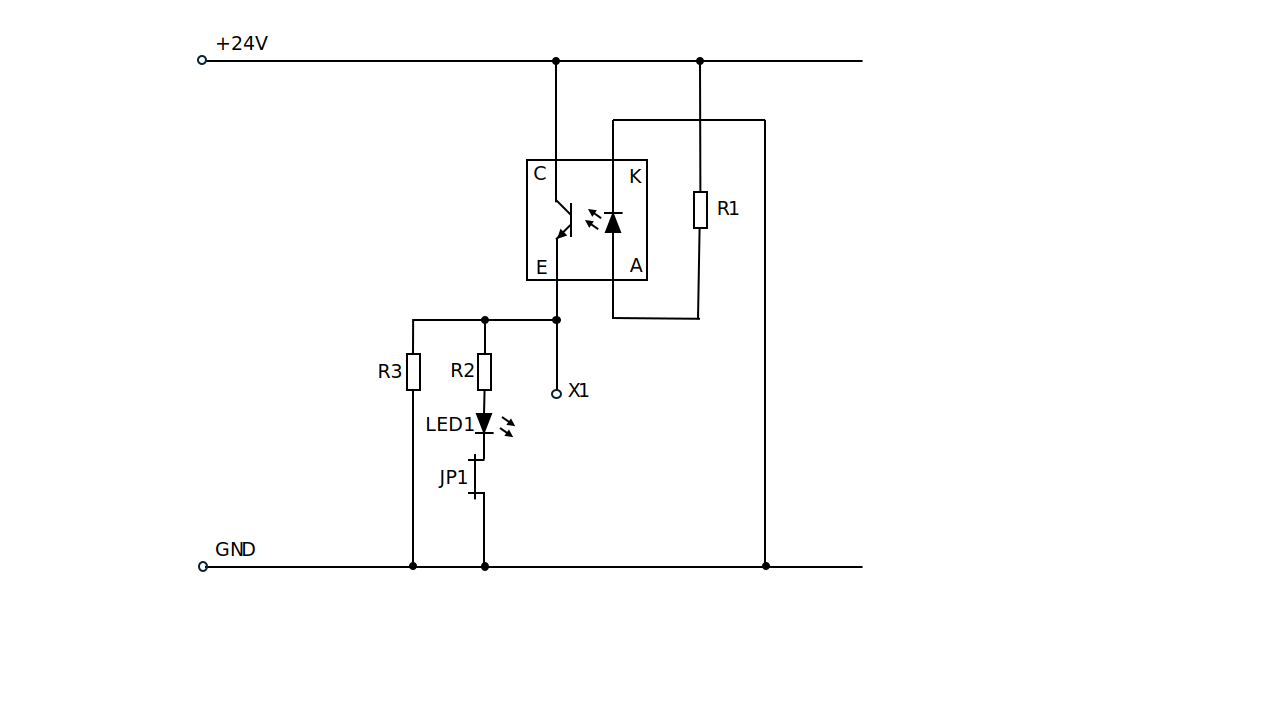
\includegraphics[width=0.6\textwidth]{Sensors/Ref_Schaltplan.png}
    \caption{Schaltplan Referenzplatine}
    \label{Ref_Schaltplan}
\end{figure}

\paragraph{Platinenentwurf und -herstellung} \mbox{}\\
Um die benötigten Referenzplatinen herstellen zu können, muss zuerst ein Leiterplattenplan in Fusion360, ehemals Eagle, erstellt werden. Über den Sharepoint der HTL lässt sich eine Elektronikbibliothek, die alle in der Schule verfügbaren Bauteile beinhaltet, herunterladen. Da der in der Schaltung verwendete Opto Interrupter nicht in der Schule verfügbar ist, sondern extern organisiert werden musst, befindet er sich nicht in dieser Elektronikbibliothek. Daher muss für ihn ein eigenes Symbol sowie ein dazugehöriger Footprint gezeichnet werden.\\
Zum Entwerfen des Printed Circuit Boards (PCB) muss ein neuer Elektronikentwurf in Fusion erstellt werden. Hier muss zuerst der zugehörige Schaltplan gezeichnet werden. Wichtig ist, dass bei der dreipoligen Schraubklemme das Bauteil 3282837-3 (J1) verwendet wird, da sonst die Abstände zwischen den Lötpads zu klein und diese zu nah bei einander sind. Damit der Jumper (JP2) nicht verloren geht, wenn die Verbindung zwischen Ground und LED aufgehoben werden soll, wird ein dreipoliger Pinheader verwendet, um den Jumper für den gegebenen Zeitraum einfach umstecken zu können.\\
Nach Fertigstellung des Schaltplans kann in Fusion ein passendes Leiterplattendokument erstellt werden, welches die Bauteile und die zugehörigen Verbindungen direkt übernimmt. Für den fertigen Leiterplattenplan des Referenztasters siehe Abb.\ref{Ref_LPPlan}. Da beim verwendeten Opto Interrupter Löcher zur Montierung vorhanden sind, müssen auf der Platine selbst keine zusätzlichen Bohrungen eingeplant werden. Bein der Anordnung der Bauteile auf der Platine ist zu beachten, dass sich die Löcher am Opto Interrupter, am schmäleren rand der Platine befinden. Um eine leichtere Verkabelung zu ermöglichen, sollte auch die Schraubklemme am Rand der Platine platziert werden.

\begin{figure}[H]
    \centering
    \includegraphics[width=0.7\textwidth]{Sensors/Ref_Leiterplattenplan.png}
    \caption{Leiterplattenplan Referenzplatine}
    \label{Ref_LPPlan}
\end{figure}

Wenn die Bauteile alle platziert und verbunden worden sind, sowie ein Polygon über die gesamte Platine gezogen worden ist, muss diese noch auf Fehler geprüft werden. Auch hier ist eine bereits fertige Datei, welche die benötigten Design Rules für Fusion360 beinhaltet, auf der Schulwebsite zu finden. Wichtig ist, damit die Platine zur Produktion in der Leiterplattenfertigung der HTL eingereicht werden kann, muss diese den vorgegebenen Anforderungen entsprechen. Dazu gehört, dass sich das HTL-Logo auf der Platine befindet und die Texteinstellungen Font: Vector, Ratio: \qty{16}{\percent} und Size: min \qty{70}{mil} entsprechen. Auch die Breite der Kupferbahnen darf nicht zu klein sein (hier: \qty{32}{mil}).\\
Nach Einreichung des Fertigungsauftrags wird die Platine von Schülerinnen und Schülern der HTL gefertigt. Der Prozess startet mit dem Reinigen des Basismaterials, um es daraufhin mit dem Negativtrockenresist (Trockenfilm) zu laminieren. In den nächsten Schritten werden die Layout-Informationen mit einem Belichter auf das Laminat übertragen und das unbelichtete Laminat mit einer Natrium-Carbonat Lösung von der Platine entfernt. Daraufhin werden durch Ätzen mit einer Eisen-III-Chlorid-Lösung strukturierte Kupferflächen freigestellt. Als Nächstes werden die Löcher in die Kupferpads gebohrt und die Platine auf ihre korrekte Größe zugeschnitten. Durch das Legen der Leiterplatte in eine Entschichtlösung aus \qty{5}{\percent}{igem} Kaliumcarbonat mit Wasser werden Ätzresiste von der Platine entfernt. Zu guter Letzt wird die Platine mit einem Versiegelunglack versiegelt, um sie vor Umwelteinflüssen und Korrosion zu schützen.

\paragraph{Platinentestung und Messung} \mbox{}\\


\subsubsection{Lichttaster}

\subsubsection{Barcode-Scanner}

\subsection{AS-Interface}

+irgendwo profibus einbauen

\subsubsection{Allgemeines}

\subsubsection{Programmierung im TIA-Portal}

\subsubsection{Verkabelung}


\subsection{Sicherheitstechnik}
\subsubsection{Grundanforderungen und Planung}
\subsubsection{Realisierung}


\newpage

\section{Anhang}
\subsection{Testergebnisse}

\subsection{Abmessungen}

\subsection{Datenblattauszüge}

\textcolor{blue}{Im Anhang befinden sich weitere Detailinformationen des Projekts wie\\
•	Datenblattauszüge, Fertigungsunterlagen (PCB-Layouts, Gehäusezeichnungen, 3D-Druckunterlagen, Montageanleitungen,…) etc.\\
•	sämtliche geforderten Projektmanagementdokumente\\
•	ein Businessplan (optional)
}

\subsection{Projektmanagement}
\textcolor{blue}{In diesem Kapitel soll auf das Projektmanagement des Projektes eingegangen werden. Zu Beginn empfiehlt es sich, die einzelnen Bereiche des Projektmanagements zu erklären und anschließend in einzelnen Kapiteln zu behandeln.}

\subsubsection{Aufgabenstellung des Gesamtprojekts}
\textcolor{blue}{Fügen Sie an dieser Stelle den Text der genehmigten Aufgabenstellung ein, der in die Diplomarbeitsdatenbank  eingegeben wurde.}

\subsubsection{Scrum-Projektplan}
\textcolor{blue}{Fügen Sie hier den vollständigen Scrum-Projektplan, wobei die Nummern der Tasks mit der Arbeitszeitaufzeichnung übereinstimmen müssen. Der Scrum-Projektplan kann auf mehrere Seiten aufgeteilt werden.}

\bgroup
    \centering
    \includegraphics[width=0.6\textwidth]{Scrum_Projektplan_mit_Tasks.png}
    \captionof{figure}{Scrum Projektplan mit Tasks}
\egroup

\newpage
\subsubsection{Terminplanung}

\newpage

\subsubsection{Arbeitspakete}

\paragraph{Maschinenbau (Simbürger)}
\begin{itemize}
    \item Konzeptionierung des Gesamtsystem
    \item CAD - Planung
    \item Komponentenfertigung
    \item Aufbau 
\end{itemize}

\paragraph{Softwareentwicklung (Simbürger)}
\begin{itemize}
    \item Benutzeroberfläche
    \item Warehouse Management System
    \item Datenbanken
\end{itemize}




\newpage

\subsection{Inbetriebnahme}
\color{blue}
Nachdem typische Projekte aus mehreren Komponenten bestehen, ist es oft nicht trivial die einzelnen Komponenten korrekt zu konfigurieren und das Gesamtsystem in Betrieb zu nehmen. In diesem Kapitel soll eine vollständige, präzise und trotzdem möglichst kompak-te Anleitung zur Inbetriebnahme des Systems dargelegt werden. Die Schritte sollen in dem Detailgrad beschrieben werden, dass ein durchschnittlicher Schüler des vierten Jahrganges das Projekt in Betrieb nehmen kann. Exemplarisch sollten Punkte wie die folgenden be-handelt werden – die Aufzählung ist nicht vollständig):
\begin{itemize}
    \item Treiberinstallationen und Systemkonfigurationen
    \item Zu empfehlen wäre bei Server-Installationen ein Setup-Script, welches auf einem vordefinierten Docker-container aufbaut.
    \item Welche Schritte sind notwendig, um das Projekt mit dem vorhandenen Code / Schaltplänen (auf GIT, CD, Netzlaufwerk, etc.) in Betrieb zu nehmen.
    \item Bei Schaltungen mit mehreren Platinen muss beschrieben werden, wie diese mit-einander verbunden werden müssen.
\end{itemize}
\color{black}

\newpage
\subsection{Kostenaufstellung}
\textcolor{blue}{Für die Kalkulation im Gesamtprojekt sind folgende Kosten zu erfassen: \\
•	Kosten für Material (Hard- und Software)\\
•	externe Kosten (z.B.: Zukauf von Sensoren, Funkmodule, spezielle Entwicklungsum-gebungen, etc.) 
}
\begin{figure}[h]
    \includegraphics[width=0.8\textwidth]{Kostenaufstellung.png}
    \centering
    \caption{Kostenaufstellung}
\end{figure}

\newpage
\subsection{Besprechungsprotokolle}
%include pdf file as image, on howl page with label
\begin{figure}[H]
    \includegraphics[width=0.9\textwidth]{../Protokolls/Projektbesprechung_0.pdf}
    \centering
    \caption{Besprechungsprotokoll 10.12.2024}
\end{figure}

\begin{figure}[H]
    \includegraphics[width=0.9\textwidth]{../Protokolls/Projektbesprechung_1.pdf}
    \centering
    \caption{Besprechungsprotokoll 16.10.2024}
\end{figure}

\begin{figure}[H]
    \includegraphics[width=0.9\textwidth]{../Protokolls/Projektbesprechung_2.pdf}
    \centering
    \caption{Besprechungsprotokoll 10.12.2024}
\end{figure}

\begin{figure}[H]
    \includegraphics[width=0.9\textwidth]{../Protokolls/Projektbesprechung_3.pdf}
    \centering
    \caption{Besprechungsprotokoll x.x.xxxx}
\end{figure}




\newpage
\subsection{Arbeitsnachweis}
\textcolor{blue}{Jedes Teammitglied (Schüler/in) hat einen vollständigen Arbeitszeitnachweis, der außer-halb des Unterrichts verrichteten Tätigkeiten, in tabellarischer Form zu erbringen. \\Eine entsprechende Vorlage wird auf den Schulrechner in Form einer Excel-Vorlage bereitgestellt.}

\begin{longtable}{|l|p{10cm}|r|}
    \hline
    \textbf{Datum} & \textbf{Tätigkeit} & \textbf{Stunden} \\
    \hline
    \endfirsthead

    \hline
    \textbf{Datum} & \textbf{Tätigkeit} & \textbf{Stunden} \\
    \hline
    \endhead

    \hline
    \endfoot

    \hline
    \endlastfoot

4.10.2023	&Besprechung des weiteren vorgehens mit WB	&0.5\\
9.10.2023&	Gruppenbesprechung für das weitere Vorgehen	&1.0\\
9.11.2023&	Reconstruction Siemens Twin Towers	&3.5\\
14.11.2023&	Reconstruction Siemens Twin Towers	&2.0\\
23.11.2023&	Reconstruction Siemens Twin Towers Lasern	&2.0\\
29.11.2023&	RSTT Ausfahrer + Schlitten Fertig&	4.0\\
19.12.2023	&CAD Auf/Ab-fahrer	&3.0\\
20.12.2023	&CAD RSTT, AutCad vorbereitung	&2.0\\

10.1.2024	&Testversuch ET200 SPS Stepdrive inkl. Meeting Knapp&	4.0\\
11.1.2024	&Achse mech. fertig, Schlitten Vertikal&	4.0\\
12.1.2024	&CAD Schuttel, Tag der offenen Tür	&2.0\\

16.1.2024	&Motor ansteuern&	1.0	\\
20.1.2024	&Umlenkungen und Aufhängungskonstruktion&	4.0\\
29.1.2024	&Diagramm Datenaustausch	&2.0\\

1.2.2024	&Besprechung WB&	4.0\\
3.2.2024	&WS Backend/Frontend Prototyp&	9.0\\
4.2.2024	&WS Frontend&	3.0\\

5.2.2024	&KWF Antrag schreiben und WS Datenbankmanagement&	3.0\\
7.2.2024	&OPC UA Client&	4.5\\
15.2.2024	&WS Suche usw, Orga, Maschinenbaubesprechung	&5.5\\

20.2.2024	&Python / OPC UA Client 	&1\\
23.2.2024	&WS Warenkorb, restructuring	&9.0\\
24.2.2024	&WS Warenkorb fertig OPC anfang und Pflichtenheft Erstversion&	6.0\\
27.2.2024	&Barcode-Scanner/http-Kommunikation	&4.0\\
28.2.2024	&Lasten/Pflichtenheft erstellen	&3.0\\


4.3.2024	&Barcode-Scanner/http-Kommunikation&	3.5\\
10.3.2024	&CAD X-Achse	&7.0\\

13.3.2024	&Absprache mit Wurnitsch bez. Pflichtenheft	&1.0\\
14.3.2024	&Barcode-Scanner/http-Kommunikation/Fusion oder so&	3.0\\
1.4.2024	&Datenbanken und Visu	&5.0\\

2.4.2024	&Lagerregal&	2.0\\
17.4.2024	&Gabel und Software&	2.0\\
23.4.2024	&STT-Fortsetzung / Software einführung&	2.5\\
12.4.2024	&Datenbanken und Visu	&5.0\\
21.4.2024	&Datenbanken und Visu	&5.0\\
22.4.2024	&cooler search stuff	&3.0\\
23.4.2024	&cooler search stuff Implementierung	&2.0\\
28.4.2024	&Areas und Locations implementierung	&6.0\\
19.4.2024	&Order stuff	&3.0\\
22.5.2024	&Order algorithmus	&3.0\\
2.6.2024	&Order api	&5.0\\
3.6.2024	&Api implement und visu	&3.0\\

4.6.2024	&STT-Fortsetzung / CAD&	2.0\\
6.6.2024	&SPS/Server Communictaion und Z-Prototyp CAD	&5.0\\
8.6.2024	&SPS Comm und Simu implement	&4.0\\
9.6.2024	&System Controler	&4.0\\

14.6.2024	&Z-Prototyp Bauteile Vorbereitung&	1.0\\
18.6.2024	&Return, Cart	&4.0\\
19.6.2024	&Docker (f me)	&3.0\\

21.6.2024	&Z-PT, Schaltschrank, SPS-Com&	4.5\\
16.7.2024	&Recherche, Ref-Elektronik&	1.0\\
17.7.2024	&Ref-Elektronik	&2.0\\
19.7.2024	&Designe/CAD rollen u. spannen y, ...	&6.0\\
22.7.2024	&Designe X-Spann	&2.0\\
25.7.2024	&Design X-Spann, Rollen	&1.5\\
31.7.2024	&Z-Achsen zauberei (sike)(doch ned)&	1.0\\
1.8.2024	&Z-Achse Redesign (sigh)	&5.0\\
9.8.2024	&YZ-Achse grobe fertigstellung&	5.0\\
10.8.2024	&YZ-Achse feinerschliff	&4.0\\
11.8.2024	&YZ-Achse + X-Achse beginn&	2.0\\
12.8.2024	&X-Achse	&1.0\\
13.8.2024	&X-Achse side roller	&4.0\\
14.8.2024	&X-Achse side roller 2. side	&2.0\\
15.8.2024	&X-Achse Mid rollers, side wheeles 90, yz-achse spiegelung	&6.0\\
16.8.2024	&YZ-Achse lichttaster, X-Achse	&1.0\\
17.8.2024	&X-Achse Schleppkettengedanken 	&6.0\\
19.8.2024	&Schleppenderketten	&2.0\\
20.8.2024	&Vertikeale Schleppkette	&3.0\\
20.8.2024	&Sponsorenemail beginn	&1.3\\
21.8.2024	&Kontaktdaten, Projektzusammenfassung	&1.5\\
22.8.2024	&Schlitten Top	&1.0\\
24.8.2024	&Stückliste, Schlitten Top	&2.0\\
25.8.2024	&X-Top Verbindung, Umlenkung	&5.0\\
27.8.2024	&Rahmen aufhängungen	&2.0\\
29.8.2024	&Umlenkungen, Motoraufhängungen	&5.0\\
30.8.2024	&Endschalter, Rahmen beginn	&3.0\\
31.8.2024	&Rahmen, Lagerschrank beginn	&6.0\\
1.9.2024	&Lagerschrank, Querfördererauschschnitt	&2.0\\
2.9.2024	&Bissi Software angeschaut wieder, cooler slider	&1.0\\
3.9.2024	&Software Richten, Weidmüller Sortiment Bauteile auswählen	&4.0\\
4.9.2024	&Stack Bug behoben, Querförderer	&7.0\\
5.9.2024	&Mech weitestgehende Fertigstellung	&4.0\\
9.9.2024	&Marketing, Fortschritts-Leafletter (+ Latex aufsetzen)	&2.5\\

10.9.2024	&Meeting Weidmüller&	2.0	\\
11.9.2024	&Schaltschrank konzeptionierung (Materialliste fast vollständig)	&2.25\\


15.9.2024	&Lapp Liste, Knapp Update, Fusion Stücklistenanfänge	&2.0\\

17.9.2024	&Autolager Demontieren für Bauteilbeschaffung&	2.5\\
18.9.2024	&Förderband Abmessen, Verbindungstest, Sensorensicherun, Suchalgorythmus Rustimplementation &6.0\\
19.9.2024	&Suchag. Fertig implementiert. Rollen gezeichnet	&3.0\\

24.9.2024	&Projektmanagement&	3.0\\
25.9.2024	&Änderungen V-Slot-Aufhängung, Project-Libre	&1.0\\

26.9.2024	&Igus, Weidmüller, Motoren ansteuern die 1.&	4.0\\
28.9.2024	&Bux im Lageralgo beheben	&1.5\\

1.10.2024	&Zeitplan, Sensoren recherchieren, SchSch-Konzept. CAD	&1.0\\
3.10.2024	&Profile bearbeiten	&1.5\\
8.10.2024	&Latex Vorlage	&1.0\\
9.10.2024	&Raumeinrichtung, SchSch Komzept&	3.0\\
21.10.2024	&Rahmenbau beginn&	2.0\\
22.10.2024	&Rahmenbauu + Drehstrom, 2.Präsentation, Auftragsvorbereitung X-Aufhängung, Referenzschaltung &5.5\\
23.10.2024	&Rahmenbau	&3.0\\
24.10.2024	&Rahmenbau, Poster/2.Präsentation	&3.0\\
25.10.2024	&XZ-Redesign	&3.0	\\
26.10.2024	&XZ-Redesign	&7.0	\\
27.10.2024	&Auftragsvorbereitung X-Achse	&3.0\\
28.10.2024	&Auftragsvorbereitung X-Achse	&2.0	\\

5.11.2024	&Beginn Umlenkrollen Drehen	&0.8\\
6.11.2024	&Weidmüller DP Inbetrtiebnahme&	1.0\\
7.11.2024	&E-Plan/Autocad, Weidmülller ansteuern&	3.5\\
8.11.2024	&E-Plan/Autocad, Weidmülller ansteuern&	3.5\\
12.11.2024	&Drehen, E-Plan, &	3.5\\
19.11.2024	&Drehen, Fräsen	&2.5\\
20.11.2024	&DAS Beg drehen	&1.0\\
21.11.2024	&DAS TFIDF	&2.0\\
22.11.2024	&Eplan, Website, SPS, Dipl Arbeit	&4.5\\
23.11.2024	&API stack umscheissen, DPWS	&3.0\\
24.11.2024	&DPWS	&2.0\\
25.11.2024	&DPWS	&1.5\\

26.11.2024	&Eplan, Website, SPS, Drehen& 3.5\\
29.11.2024	&Eplan, Website/Referenzplatine, Blockschaltbild, Dipl Arbeit& 4.0\\
3.12.2024	&Drehen,ASI-Sensoren-Platine, Diplomarbeit, DA Maschinenbau& 5.0\\
6.12.2024	&Website, DA &3.5\\
10.12.2024	&DA, Fusion, ASi in E-Plan, DA software	&5.0\\
13.12.2024	&E-Plan &3.5\\
7.1.2025	&Website, SchSch, SPS, CNC-Fräsen, Hülsen Drehen&	3.5\\
8.1.2025	&X-Achse Zusammenbauen anfangen	&2.0\\
10.1.2025	&CAD für Schaltschrankmodule, ZB	&4.0\\
14.1.2025	&Zusammenbauen, SPS, …&	4.0\\
15.1.2025	&ZB, Kabel verlegen, Platinen löten&	4.5\\
17.1.2025	&Tag der offenen Türe	&5.0\\
21.1.2025	&Schaltschrank, TIA Portal, ?&	3.5\\
24.1.2025	&Lasern, Förderband, Mechanik	&3.5\\
4.2.2025	&Sicherheitstechnik-Besprechung, SPS <--> Server	&3.5\\
14.2.2025	&WMS Location Updateing	&1.0\\
17.2.2025	&DA allgem	&1.0\\

21.2.2025	&Ref, Fräsen, Da-Schreiben	&5.0\\
25.2.2025	&Zusammenbauen&	4.0\\
28.2.2025	&Fräsen, E-Plan,&	3.5\\
2.3.2025	&DA aufbau	&1.5\\
3.3.2025	&DA - Besprechungsprotokolle&	1.0\\

5.3.2025	&Umlenkung + Motoren&	4.5\\
6.5.2025	&DA-Schreiben  &	2.5\\
9.3.2025	&DA - yz	&1.0\\

10.3.2025	&DA-schrieben	&3.0\\
11.3.2025	&DA-schreiben	&3.0\\
14.3.2025	&Verkabelung Schaltschrank	&4.0\\


    
\end{longtable}


\newpage


\newpage
\addcontentsline{toc}{section}{Literaturverzeichnis}
\printbibliography[title=Literaturverzeichnis]

\newpage
\renewcommand{\cftfigpresnum}{Abb. }
\setlength{\cftfignumwidth}{2cm}
\listoffigures

\newpage

\renewcommand{\cfttabpresnum}{Tab. }
\setlength{\cfttabnumwidth}{2cm}
\listoftables

\end{document}